\documentclass{sig-alternate}
\graphicspath{{graphics/}}

\DeclareGraphicsExtensions{.eps,.pdf,.png,.jpg,.mps}

\hyphenation{maxStackSize eventXCS}
\usepackage[scriptsize,hang]{subfigure}
\usepackage{mdwlist}
\usepackage{stkernel}
\usepackage[T1]{fontenc}

\begin{document}
\conferenceinfo{GECCO'10,} {July 7--11, 2010, Portland, Oregon, USA.} 
\CopyrightYear{2010}
\crdata{978-1-4503-0072-8/10/07}
\clubpenalty=10000
\widowpenalty = 10000 

\title{Adaption of XCS to Multi-Learner Predator/Prey Scenarios}

%\subtitle{[Track: Genetics Based Machine Learning]}

\numberofauthors{3}

 \author{
	\alignauthor
		Clemens Lode \\
    \affaddr{Karlsruhe Institute of Technology} \\
    \affaddr{Institute AIFB} \\
    \affaddr{76128 Karlsruhe, Germany} \\
  	\email{clemens@lode.de}
	\alignauthor
		Urban Richter \\
    \affaddr{Karlsruhe Institute of Technology} \\
    \affaddr{Institute AIFB} \\
    \affaddr{76128 Karlsruhe, Germany} \\
    \email{urban.richter@kit.edu} \\
	\alignauthor
		Hartmut Schmeck \\
   \affaddr{Karlsruhe Institute of Technology} \\
   \affaddr{Institute AIFB} \\
   \affaddr{76128 Karlsruhe, Germany} \\
   \email{hartmut.schmeck@kit.edu}
}

\date{4 April 2010}

\maketitle

%\begin{abstract}

% This paper investigates an approach of concurrent learners, where the credit assignment problem is specially addressed (How to divide team reward among the individuals?). Moreover, the investigated approach is focussed on the dynamics of learning (How to cope with the problem of coadaptation?) in an instance of the homogeneous and (non-) communicating predator/prey scenario. To compensate the dynamic nature of such a scenario, a new algorithm is developed \emph{(SXCS)} by modelling the reward function according to an heuristic with high performance and by using memory to record and analyze the movements and the history of function's past values. 

Learning classifier systems (LCSs) are rule-based evolutionary reinforcement learning systems. Today, especially variants of Wilson's \emph{eXtended classifier system (XCS)} are widely applied for machine learning. Despite their widespread application, LCSs have drawbacks, e.\,g., in multi-learner scenarios, since the \emph{Markov property} is not fulfilled. In such scenarios, typical challenges of research are: How to divide team reward among the individual learners and how to cope with the problem of parallel learning agents (coadaptation)?

In this paper, an instance of the generic homogeneous and (non-) communicating predator/prey scenario is used to adapt an XCS to such a scenario with concurrent and cooperating learners. Results show that improvements in learning can be achieved by cleverly adapting the \emph{multi-step} approach to the characteristics of the investigated scenario. Firstly, the environmental reward function is expanded to include sensory information. Secondly, the learners are equipped with a memory to store and analyze the history of local movements and given payoffs. 

% The predator/prey domain is an appropriate example that has successfully been studied in a variety of instantiations. It does not serve as a complex real world domain, but as a test scenario for demonstrating and evaluating manifold research ideas. 

\end{abstract}


\begin{abstract}

Learning classifier systems (LCSs) are rule-based evolutionary reinforcement learning systems. Today, especially variants of Wilson's \emph{extended classifier system (XCS)} are widely applied for machine learning. Despite their widespread application, LCSs have drawbacks, e.\,g., in multi-learner scenarios, since the \emph{Markov property} is not fulfilled. 

In this paper, LCSs are investigated in an instance of the generic homogeneous and non-communicating predator/prey scenario. A group of predators collaboratively observe a (randomly) moving prey as long as possible, where each predator is equipped with a single, independent XCS. Results show that improvements in learning are achieved by cleverly adapting a \emph{multi-step} approach to the characteristics of the investigated scenario. Firstly, the environmental reward function is expanded to include sensory information. Secondly, the learners are equipped with a memory to store and analyze the history of local actions and given payoffs.

\end{abstract}

\category{I.5.2}{Design Methodology}{Classifier design and evaluation}
\terms{Algorithms, Theory}

\keywords{Agent cooperation, evolutionary learning, XCS, multi-agent learning, coordination task, non-Markovian environments}

%\section{Introduction}
\label{section:introduction}

The complexity of today's technical systems is continuously increasing. Future systems will consist of a multitude of autonomous soft- and hardware components that interact with each other to satisfy functional requirements of the global system. Since this trend bears the risk of unpredictable or even uncontrollable system behavior, \emph{organic computing} \cite{RMB+06} % \cite{Sch05b} % \footnote{http://www.organic-computing.de/spp} % {We gratefully acknowledge the financial support by the German Research Foundation (DFG) within the priority programme 1183 Organic Computing.} 
focuses on monitoring, analyzing, and controlling complex distributed systems to endow them with the ability of \emph{controlled self-organization}. An or\-ga\-nic system can self-organize to achieve its tasks while being simultaneously observed and, if necessary, influenced by a higher level component to avoid unwanted emergent system states. To this end, an \emph{observer/controller architecture} has been proposed in \cite{RMB+06}. % that monitors and analyses the status of a \emph{system under observation and control} and influences its behaviour. 
Since it is in general impossible to foresee all possible configurations the \emph{system under observation and control} takes on in a dynamic environment, it is important to endow the system with \emph{learning components} so that system components can autonomously learn new control actions for unforeseen situations and evaluate their consequences. An XCS \cite{Wil95} is a rule-based evolutionary on-line learning system that is suitable to perform this learning task. It evolves a set of condition-action-mappings (called \emph{classifiers}) that contain a reward prediction estimating the benefits of their action for situations matching their condition. 
%new
In general, LCSs combine aspects of evolutionary algorithms, which are used for rule generation, with reinforcement learning, which is used for reward prediction (e.\,g., if an agent reaches a goal, a reward will be distributed among the classifiers). 
%In general, LCSs combine aspects of evolutionary algorithms that are used for rule generation with reinforcement learning that is used for reward prediction. I.\,e., if an agent reaches a goal, a reward will be distributed among the classifiers. 
Usually, this depends on the type of scenario: In \emph{single-step} environments, a reward is generated at each learning iteration, while in \emph{multi-step} environments (which are often characterized by local and restricted knowledge) 
%new
multiple steps are usually required to solve a problem and to generate a reward.
%the agent will construct the global information about the best classifiers % condition-action-mapping 
%using multiple % repetitions and 
%iterations of the whole learning problem.

Here, LCSs are used to learn control rules for agents in a \emph{predator/prey scenario}~\cite{BJD86}. Following the global task to observe one or up to $n$ (randomly) moving preys, a number of predators has % have
to achieve a common goal with local and distributed behavior (i.\,e., maximizing the global \emph{observation time}). The scenario shows technical relevance to organic computing scenarios concerning the learning aspect, it seems to be very flexible in its parametrization, and it allows many variations \cite{SV00}. % : Depending on the playground the agents have to live in, implementations can vary the number of agents, the number of targets, the number and distribution of obstacles, the moving strategies, the learning behaviour of the agents, the definition of local neighbourhoods, the communication possibilities between the agents, and various forms of collaboration and collective learning could be analysed. 
%E.\,g., agents can learn strategies for any given group behavior and they can exchange locally learned knowledge -- to benefit from their swarming behavior or to adapt quicker than in a single-agent case. 
Thus, the challenge of concurrent learning agents is specially addressed, where all predators are equipped with a single, independent XCS.
% In this paper a predator/prey scenario~\cite{BJD86} in the connection with a learning classifier system (LCS) is examined. Following the global task to observeone or up to $n$ (randomly) moving targets/preys, a number of rovers/predators has to achieve a common goal with local and distributed behaviour, e.\,g., maximizing the global observation time or catching moving target(s). The scenario shows technical relevance to Organic Computing scenarios and it seems to be very flexible in its parametrisation. Especially, it allows many variations: Depending on the playground the agents have to live in, implementations can vary the number of agents, the number of targets, the number and distribution of obstacles, the moving strategies, the learning behaviour of the agents, the definition of local neighbourhoods, the communication possibilities between the agents, and various forms of collaboration and collective learning could be analysed. 
% E.\,g., agents can learn strategies for any given group behavior and they can exchange locally learned knowledge -- to benefit from their swarming behavior or to adapt quicker than in a single-agent case. Here, the challenge of concurrent learning agents is addressed, where all agents are equipped with a single, independent LCS. 
%cf.\current field of research in the field of LCSs are the so-called \emph{eXtended Classifier Systems} (XCS)~\cite{Butz2006}\cite{BW02}\cite{Wil95}. Basically an XCS is a LCS, i.\,e., a number of rules, so-called \emph{classifiers}), each consisting of a condition/action pair. When the sensors of an agent match a condition then the action is executed. As wild-cards can be part of the condition a mechanism usually has to select from multiple classifiers. The classifiers are updated and adapted to the environment step by step using \emph{reinforcement learning}. When an agent reaches a goal condition a reward is distributed among the classifiers. The way this is done usually depends on the type of scenario, in a single-step environment a reward is generated at each step while in a multi-step environment with local information the agent has to construct the global information using multiple repetitions and steps.
Since neither the classical single-step nor the multi-step implementation of an XCS \cite{BW02} can be used to learn a \emph{dynamic observation task} % in a predator/prey scenario with obstacles 
(see argumentation in Section~\ref{subsection:scenario-classification}), the special focus of this paper is on an approach, how to handle such dynamic predator/prey scenarios. Thereby, the proposed idea is mainly based on a \emph{local cooperative reward function} and some kind of a \emph{temporary memory}. This memory stores a number of past action sets and their corresponding reward values. 
%new
Although LCSs have been investigated in dynamic environments \cite{Lan98,LW00}, specifically predator/prey scenarios have not really been addressed in XCS literature. % While there are works about LCSs in dynamic environments \cite{Lan98,LW00} specifically predator/prey scenarios have not really been addressed in XCS literature. % The discussion of such scenarios is an addition to existing literature about XCSs in dynamic scenarios  because predator/prey scenarios have not really been addressed in XCS literature.

% using \emph{not} global communication and organisation, e.\,g., as presented in \cite{TTS01}. % While there are implementations to handle such scenarios, they are either very simple with a goal object that can only be moved by agents, with only one or two agents and no obstacles~\cite{1102281} or use global communication and organization with a shared global classifier set~\cite{TTS01}.

% Thus, a promising modified XCS approach has been investigated to overcome the drawbacks of the classical XCS algorithm. The proposed idea is mainly based on a local cooperative reward function and some kind of temporary memory, which stores past actions sets and their corresponding reward values. Thus, local payoffs can be delayed and the reward function reflects in a better way the local agent behaviour. Cooperation (incorporated in the reward function) is more or less achieved through rejection and attraction. Predators reject each other, the prey attracts the predators. Thus, agents try to uniformly distribute on the grid and observation time of the prey seems to be maximized. In addition it is shown that the new XCS approach retains its ability to recognize local obstacle configurations in order to reach the goal object.

Thus, the remainder of this paper is structured as follows: First, LCSs are shortly introduced and their usability in different scenarios is discussed in Section~\ref{section:learning-classifier-systems}. 
%In Section~\ref{section:the-predator-prey-example}, the predator/prey example is described, which has not really been addressed in XCS literature as yet. %(in connection with XCS) new type of scenario (see Section~\ref{section:the-predator-prey-example}) is then presented and classified. 
Additionally, the characteristics of a predator/prey scenario are presented, which require a new reward function, as introduced in Section~\ref{section:the-reward-function}. Using this new reward function, several experiments are executed according to the methodology, as described in Section~\ref{section:methodology}. Experimental results are presented in Section~\ref{section:experimental-results}. The paper concludes with a summary and a discussion of future work in Section~\ref{section:conclusion}. % The paper concludes with Section~\ref{section:conclusion} with the result that the new approach shows significant improvements over the standard implementation but still need further research.


\section{Introduction}
\label{section:introduction}

The complexity of today's technical systems is continuously increasing. Future systems will consist of a multitude of autonomous soft- and hardware components that interact with each other to satisfy functional requirements of the global system. Since this trend bears the risk of unpredictable or even uncontrollable system behavior, \emph{organic computing} \cite{RMB+06} % \cite{Sch05b} % \footnote{http://www.organic-computing.de/spp} % {We gratefully acknowledge the financial support by the German Research Foundation (DFG) within the priority programme 1183 Organic Computing.} 
focuses on monitoring, analyzing, and controlling complex distributed systems to endow them with the ability of \emph{controlled self-organization}. An or\-ga\-nic system can self-organize to achieve its tasks while being simultaneously observed and, if necessary, influenced by a higher level component to avoid unwanted emergent system states. To this end, an \emph{observer/controller architecture} has been proposed in \cite{RMB+06}. % that monitors and analyses the status of a \emph{system under observation and control} and influences its behaviour. 
Since it is in general impossible to foresee all possible configurations the \emph{system under observation and control} takes on in a dynamic environment, it is important to endow the system with \emph{learning components} so that system components can autonomously learn new control actions for unforeseen situations and evaluate their consequences. An XCS \cite{Wil95} is a rule-based evolutionary on-line learning system that is suitable to perform this learning task. It evolves a set of condition-action-mappings (called \emph{classifiers}) that contain a reward prediction estimating the benefits of their action for situations matching their condition. 
%new
In general, LCSs combine aspects of evolutionary algorithms, which are used for rule generation, with reinforcement learning, which is used for reward prediction (e.\,g., if an agent reaches a goal, a reward will be distributed among the classifiers). 
Usually, this depends on the type of scenario: In \emph{single-step} environments, a reward is generated at each learning iteration, while in \emph{multi-step} environments (which are often characterized by local and restricted knowledge) 
%new
multiple steps are usually required to solve a problem and to generate a reward.

Here, LCSs are used to learn control rules for agents in a \emph{predator/prey scenario}~\cite{BJD86}. Following the global task to observe one or up to $n$ (randomly) moving preys, a number of predators has % have
to achieve a common goal with local and distributed behavior (i.\,e., maximizing the global \emph{observation time}). The scenario shows technical relevance to organic computing scenarios concerning the learning aspect, it seems to be very flexible in its parametrization, and it allows many variations \cite{SV00}.
Thus, the challenge of concurrent learning agents is specially addressed, where all predators are equipped with a single, independent XCS.

Since neither the classical single-step nor the multi-step implementation of an XCS \cite{BW02} can be used to learn a \emph{dynamic observation task} % in a predator/prey scenario with obstacles 
(see argument in Section~\ref{subsection:scenario-classification}), the special focus of this paper is on an approach, how to handle such dynamic predator/prey scenarios. The proposed idea is mainly based on a \emph{local cooperative reward function} and some kind of a \emph{temporary memory}. This memory stores a number of past action sets and their corresponding reward values. 
%new
Although LCSs have been investigated in dynamic environments \cite{Lan98,LW00}, specifically predator/prey scenarios have not really been addressed in XCS literature. % While there are works about LCSs in dynamic environments \cite{Lan98,LW00} specifically predator/prey scenarios have not really been addressed in XCS literature. % The discussion of such scenarios is an addition to existing literature about XCSs in dynamic scenarios  because predator/prey scenarios have not really been addressed in XCS literature.


Thus, the remainder of this paper is structured as follows: First, LCSs are shortly introduced and their usability in different scenarios is discussed in Section~\ref{section:learning-classifier-systems}. 
%In Section~\ref{section:the-predator-prey-example}, the predator/prey example is described, which has not really been addressed in XCS literature as yet. %(in connection with XCS) new type of scenario (see Section~\ref{section:the-predator-prey-example}) is then presented and classified. 
Additionally, the characteristics of a predator/prey scenario are presented, which require a new reward function, as introduced in Section~\ref{section:the-reward-function}. Using this new reward function, several experiments are executed according to the methodology, as described in Section~\ref{section:methodology}. Experimental results are presented in Section~\ref{section:experimental-results}. The paper concludes with a summary and a discussion of future work in Section~\ref{section:conclusion}. % The paper concludes with Section~\ref{section:conclusion} with the result that the new approach shows significant improvements over the standard implementation but still need further research.

%\section{Learning Classifier Systems}
\label{section:learning-classifier-systems}

The field of LCSs, introduced in the 1970ies \cite{Hol75,Hol76,HR78}, is one of the most active and best-developed form of genetic based machine learning \cite{Kov02a,KL00,Lan08}. As mentioned above, much of LCS's theory is inherited from the reinforcement learning literature. % The following section provides a brief overview what an LCS is. 

LCSs are rule-based on-line learning systems that combine nature-inspired optimization heuristics and reinforcement learning techniques to learn appropriate actions for any input they get \cite{Wil95}. They are applicable to any problem, where a numerical reward reflecting the quality of an action can be obtained. The core component of an LCS is its \emph{rule base} that contains rules (called \emph{classifiers}) consisting of a condition, an action, a prediction value, etc. The selection of an appropriate action for a given input is a two-step process. From the rule base of all classifiers a subset called \emph{match set} is computed that contains all classifiers, whose condition matches the current input. Then, for all distinct actions present in the match set the average prediction of all classifiers advocating the same action is calculated. The action with the highest average prediction is selected for execution and all classifiers in the match set advocating that action form the \emph{action set}. The reward received from the environment is subsequently used to update the prediction values of all classifiers in the action set.

Classifiers forming the rule base are created in two different ways: Whenever the match set is empty, classifiers consisting of a condition matching the current input, a random action, and a default prediction value are inserted into the rule base by a process called \emph{covering}. Furthermore, a randomized \emph{evolutionary component} occasionally selects relatively good classifiers to be the parent individuals for a reproduction cycle. Crossover and mutation are applied to copies of the parents to form offspring, which are inserted into the rule base. 

A variety of different LCS implementations has been proposed (cf.~\cite{Kov02a}), many are based on Wilson's XCS \cite{Wil95} system, which is an LCS implementation that maintains separate prediction and fitness values and where the fitness of a classifier is based on the \emph{accuracy} of the prediction reward.  
% While Wilson originally used a binary input encoding for XCS, different approaches to represent real-valued inputs have been examined (e.\,g., \cite{DAL05a}). % (\eg, \cite{DAL05a,SB03,Wil00a}).

% The architecture of an LCS is simple to study and the knowledge is encoded and stored in so-called \emph{classifiers}. These classifiers consist of a condition part, which is matched against the input from the environment, an action part, and some kind of fitness or strength value.

% The strength value is used to decide, which classifier should be chosen if more than one classifier matches the current input. The encoding of conditions is done in such a way that different levels of \emph{generality} are possible, hence the range of input values each classifier matches against may vary from a single point to the entire search space. In a step that is called \emph{rule discovery} new classifiers are generated using genetic operators, like crossover and mutation, on existing classifiers, changing both condition and action. Furthermore, every time no classifier matching the current input is available, one or more classifiers with a matching condition and randomly chosen action are created (this is called \emph{covering}).

% After a classifier has been generated, the system has to determine its strength value. Every time a classifier's action is chosen, the strength value of this classifier is updated using some objective function. 

In certain problems (see Section~\ref{subsection:single-step-vs-multi-step-problems}), the environment's reaction on an action executed by an LCS is not instantaneous. Thus, further reinforcement learning cycles are required to build up an optimal (local) reward function (see Section~\ref{subsection:learning-markov}). Also, more complex scenarios with aliasing positions require additional handling like an internal memory (see Section~\ref{subsection:non-markov-environments}). In dynamic scenarios, e.\,g., the predator/prey scenario, additional measures are required. This will be subject of the following sections.

% The simplest way to increase performance would be to try and find classifiers, which maximize the objective function's value. Another approach more suitable for complex problems is the use of three distinct components as \emph{strength value}: The prediction $p$ of the objective function's value after this classifier's action has been executed, the average error of this prediction $\epsilon$, and a fitness value $F$ computed from this prediction error. The prediction is used to choose an action for execution: The classifier with best prediction, weighted by its fitness, is likely to result in best performance. Furthermore, the fitness is used to find classifiers suitable as input for the generation of new classifiers using genetic operators. The goal is to represent the entire search space with as few classifiers as possible while keeping only those that are more \emph{accurate} in their prediction. This approach is realized in \emph{XCS, the eXtended Classifier System} \cite{Wil95}, which is used within this paper and described in \cite{But00,BW02}.

\subsection{Single-Step vs.\ Multi-Step Problems}
\label{subsection:single-step-vs-multi-step-problems}

Literature about LCSs could be divided into \emph{single-step} and \emph{mul\-ti-step} approaches. This separation bases on how to solve the reinforcement learning problem and addresses a design decision, which has to be taken when implementing an LCS. It refers to the question, \emph{when} a reinforcement signal (reward) is achieved from the environment and \emph{how} this reward is distributed on the past action(s). 

In \emph{single-step} environments, the external reward is received on every time step and the environmental input for each time step has completely been independent of the prior time step in the case of environments with only a single entity with an LCS. When a decision is made, the reinforcement is directly received and measures the quality of the decision. Single-step environments generally involve categorization of data examples. A typical single-step benchmark problem is the \emph{boolean multiplexer problem} \cite{BKLW04,Wil95}. 

In \emph{multi-step} environments, the external reward may not necessarily be received on any time step, since the environmental input on a time step depends on at least the prior input and the system's last action. Typical multi-step environments are known as sequential environments or so-called \emph{Maze} problems, e.\,g., \emph{Wood1}~\cite{Wil94} or \emph{Wood2}~\cite{Wil95}. These examples model the adaptive interaction of an agent with its environment and have been studied using a variety of methods. Most often, a Maze is defined as a given number of neighboring cells in a grid-world. A cell is a bounded space formally defined and is the elementary unit of a Maze. Cells are either empty or can contain an obstacle, food, a so-called \emph{animat}, and eventually a predator of the animat. 

An animat is randomly placed in the Maze environment (which could be some kind of a labyrinth) and it tries to set its position to a cell containing food, which is sparsely located in the environment. To perform this task, it possesses a limited perception of the environment (often limited to the eight cells surrounding the animat's position) and it can also only move to an empty neighboring cell. Moving step by step through the Maze in order to fulfil its goal, the animat searches for a strategy (or adopt a policy), which minimizes the effort undertaken to find the food in the selected Maze environment. Maze environments offer plenty of parameters that allow to evaluate the complexity of a given system and also to evaluate the efficiency of a learning method. A full description of these parameters is available in \cite{BZ05}.

\subsection{Learning in Markov Environments} % with Markov Property}
\label{subsection:learning-markov}

When the environment in question does have the Markov property, i.\,e., it is an environment, where the sensory data for an agent differs for each position, then an agent can acquire global information by visiting all positions of the environment. With this information, an LCS can find the optimal set of rules to find the goal on the shortest route from any starting position. The learning process itself is done by a random walk (the \emph{explore} phase) in order to cover the search space, starting from a random position and repeating the process when reaching the goal position. Actions that lead to the goal are positively rewarded. Each action is rewarded by a portion of the reward value of the next action (or the maximal reward value when reaching the goal). The actual quality (the shortness of the path length) of the LCS is determined in the next phase (the \emph{exploit} phase), where the agent only chooses actions with the highest product out of fitness and prediction values.

\subsection{Non Markov Environments}
\label{subsection:non-markov-environments}

Some Maze problems offer perceptually identical situations that require different actions to reach the food. This problem is often studied in the context of \emph{non Markov environments}. \emph{Woods101} (see Figure~\ref{figure:woods101a}) is a typical example of a \emph{partially observable Markov decision process (POMDP)}, where a \emph{single-agent} cannot distinguish different situations due to a lack of global environmental information. 

The animat is placed in a free random field, it can sense the eight adjacent cells, and has to learn to reach the food denoted with $F$, while trees $T$ blocking any movement. Here, the aliasing positions marked with 1 and 2 share the same sensory configuration, but require different optimal actions (cf.\ Figure~\ref{figure:woods101b}, each optimal action for the different positions is marked with an arrow). In position 1, the optimal action is to move to the bottom right, while the optimal action in position 2 is to move to the bottom left. Thus, an XCS cannot evolve an optimal policy for \emph{Woods101} (without further modifications).

I.\,e., using records of past condition-action-mappings by adding temporary memory is a widespread approach to cope with such environments, as investigated in \cite{Lan98,LW00}.

\begin{figure}[ht]
  \subfigure[The aliasing positions are marked with 1 and 2.]{
  	\label{figure:woods101a}
  	\includegraphics[width=0.22\textwidth]{woods101a.eps}}\hfill
  \subfigure[Sensory configuration of the two aliasing positions]{
  	\label{figure:woods101b}
  	\includegraphics[width=0.22\textwidth]{woods101b.eps}}\hfill
  \caption{\mathversion{bold}The \emph{Woods101} environment: Trees are marked with $T$, food is marked with $F$.}
  \label{figure:woods101}
\end{figure}

A second non Markov property is still embedded in \emph{multi-agent} environments and this is related to a change of an agent's internal state. In scenarios with more than one learning agent, an agent has to evaluate actions that may be caused by its own internal state or that are the result of other agent's actions. It is difficult to recognize an environmental change, which is caused by the change of another agent's internal state, due to a lack of the other agents' informations. Even if an agent stays in the same location, the agent cannot evaluate the environmental changes. In \cite{TTS01}, this second non Markov property is defined as the \emph{non observable Markov decision process (NOMDP)}. 

In Section~\ref{subsection:scenario-classification}, it will be shown that the predator/prey scenario, presented in the following and used as testbed in this paper, includes both non Markov properties (POMDP and NOMDP). Thus, learning in such environments is more complex than learning in single-agent environments (where only one agent adapts to its dynamically changing environment) and requires a different approach, which is discussed in Section~\ref{section:the-reward-function}.


\section{Learning Classifier Systems}
\label{section:learning-classifier-systems}

The field of LCSs, introduced in the 1970ies \cite{Hol75,Hol76,HR78}, is one of the most active and best-developed form of genetic based machine learning \cite{Kov02a,KL00,Lan08}. As mentioned above, much of LCS's theory is inherited from the reinforcement learning literature. The following section provides a brief overview what an LCS is. 

Hence, LCSs are rule-based on-line learning systems that combine nature-inspired optimization heuristics and reinforcement learning techniques to learn appropriate actions for any input they get \cite{Wil95}. They are applicable to any problem, where a numerical reward reflecting the quality of an action can be obtained. The core component of a LCS is its \emph{rule base} that contains rules (called \emph{classifiers}) consisting mainly of a condition, an action, and a prediction value. The selection of an appropriate action for a given input is a two-step process. From the rule base of all classifiers a subset called \emph{match set} is computed, which contains all classifiers whose condition matches the current input. Then, for all distinct actions present in the match set, the average prediction of all classifiers advocating the same action is calculated. After that an action is selected either randomly or with a probability depending on the average prediction and classifiers that advocate that action form the \emph{action set}. Finally, the reward received from the environment is subsequently used to update the prediction values of all classifiers in the corresponding action set.

Classifiers forming the rule base are created in two ways: Whenever the match set is empty, classifiers are inserted into the rule base by a process called \emph{covering}, which consists of a condition that matches the current input, a random action, and a default prediction value. Furthermore, a randomized \emph{evolutionary component} occasionally selects % relatively 
good classifiers to be the parent individuals for a reproduction cycle. Crossover and mutation are applied to copies of the parents to form offspring, which is inserted into the rule base. A variety of different LCS implementations has been proposed (cf.~\cite{Kov02a}), many are based on Wilson's XCS \cite{Wil95} system, which is an implementation that maintains separate prediction and fitness values and where the fitness of a classifier is based on the \emph{accuracy} of the prediction reward.  % While Wilson originally used a binary input encoding for XCS, different approaches to represent real-valued inputs have been examined (e.\,g., \cite{DAL05a}). % (\eg, \cite{DAL05a,SB03,Wil00a}).

In certain problems (see Section~\ref{subsection:single-step-vs-multi-step-problems}), the environment's reaction to an action executed by an LCS is not instantaneous. Thus, further reinforcement learning cycles are required to build up an optimal (local) reward function (see Section~\ref{subsection:learning-markov}). Also, more complex scenarios with \emph{aliasing positions} require additional handling like an internal memory (see Section~\ref{subsection:non-markov-environments}). In dynamic predator/prey scenarios, additional measures are required, as discussed in the following.

\subsection{Single-Step vs.\ Multi-Step Problems}
\label{subsection:single-step-vs-multi-step-problems}

Literature about LCSs could be divided into \emph{single-step} and \emph{mul\-ti-step} approaches. This separation is based on how to solve the reinforcement learning problem and addresses a design decision, which has to be taken when implementing an LCS. It refers to the question, \emph{when} a reinforcement signal (reward) is received from the environment and \emph{how} this reward is distributed on the past action(s). 

In \emph{single-step} environments having a single (centralized) learning instance, the external reward is received on every time step and the environmental input for each time step has completely been independent of the prior time step. % in the case of environments with only a single entity with an LCS.
When a decision is made, the reinforcement is directly received and measures the quality of the decision. Single-step environments generally involve categorization of data examples. A typical single-step benchmark problem is the \emph{boolean multiplexer problem} \cite{BKLW04,Wil95}. 

In \emph{multi-step} environments, the external reward may not necessarily be received on any time step, since the environmental input on a time step depends on at least the prior input and the system's last action. Typical multi-step environments are known as sequential environments or so-called \emph{Maze} problems ( e.\,g., \emph{Wood1}~\cite{Wil94} or \emph{Wood2}~\cite{Wil95}). These examples model the adaptive interaction of a single agent with its static environment and have been studied using a variety of methods. Most often, a Maze is defined as a given number of neighboring cells in a grid-world. A cell is a bounded, formally defined space and it is the elementary unit of a Maze. Cells are either empty or can contain an obstacle, food, a so-called \emph{animat}, or a predator of the animat. Then, an animat is randomly placed in the Maze environment (which could be some kind of labyrinth) and it tries to set its position to a cell containing food, which is sparsely located in the environment. To perform this task, it possesses a limited perception of the environment (often limited to the eight cells surrounding the animat's position) and it can also move to an empty neighboring cell. Moving step by step through the Maze in order to fulfill its goal, the animat searches for a strategy (or adopts a policy), which minimizes the effort undertaken to find the food in the selected Maze environment. Maze environments offer plenty of parameters that allow to evaluate the complexity of a given system and the efficiency of a learning method (cf.~\cite{BZ05}).

\subsection{Learning in Markov Environments} % with Markov Property}
\label{subsection:learning-markov}

When the sensory data from the view of an agent differs for each position in the investigated Maze environment, the Markov property is fulfilled (i.\,e., an agent can acquire global information to solve the whole learning problem by visiting all positions of the environment). Having global information, an LCS can learn the optimal set of rules to find the goal position from any starting position by computing the shortest route. The learning process itself is done by a random walk (the \emph{explore phase}) in order to cover the search space, starting from a random position and repeating the process when reaching the goal position. Actions that lead to the goal position are positively rewarded by the maximal reward value. Other actions are rewarded by a portion of the reward value of the next action. Then, the actual quality (the shortness of the path length) of the LCS is determined in the \emph{exploit phase}, where the agent only chooses actions with the highest product out of fitness and prediction values (\emph{best selection}).


\subsection{Non-Markov Environments}
\label{subsection:non-markov-environments}

\begin{figure}[ht]
  \subfigure[1 and 2 mark the two aliasing positions.]{
  	\label{figure:woods101a}
  	\includegraphics[width=0.22\textwidth]{woods101a}}\hfill
  \subfigure[Sensory configuration of the two aliasing positions]{
  	\label{figure:woods101b}
  	\includegraphics[width=0.22\textwidth]{woods101b}}\hfill
  \caption{\mathversion{bold}The \emph{Woods101} environment: Trees are marked with $T$, food is marked with $F$.}
  \label{figure:woods101}
\end{figure}

Some Maze problems offer perceptually identical situations that require different actions to reach the food. This problem is often studied in the context of \emph{non-Markov environments}. \emph{Woods101} (see Figure~\ref{figure:woods101a}) is a typical example of a \emph{partially observable Markov decision process (POMDP)}, where an animat cannot distinguish different situations due to a lack of global environmental information. 

The animat is placed in a free random field (it can sense the eight adjacent cells) and has to learn to reach the food denoted with $F$, while trees $T$ blocking any movement. Here, the aliasing positions, marked with 1 and 2, share the same sensory configuration, but require different optimal actions (see Figure~\ref{figure:woods101b}, each optimal action for the different positions is marked with an arrow). In position 1, the optimal action is to move to the bottom right, while the optimal action in position 2 is to move to the bottom left. Thus, an XCS cannot evolve an optimal policy for \emph{Woods101} (without further modifications). Using records of past condition-action-mappings by adding temporary memory is a common approach to cope with such environments, see \cite{Lan98,LW00}.

A second non-Markov property is still embedded in \emph{multi-agent} environments and this is related to a change of an agent's internal state. In scenarios with more than one learning agent, an agent has to evaluate actions that may be caused by its own internal state or that are the result of other agent's actions. It is difficult to recognize an environmental change, which is caused by the change of another agent's internal state, due to a lack of the other agent's information. Even if an agent stays in the same location, the agent cannot evaluate the environmental changes. Moreover, memory-based approaches will fail, since any memory, which stores information about the environment, becomes invalid after each step. This second non-Markov property is often defined as a \emph{non-observable Markov decision process (NOMDP)}, see~\cite{TTS01}.

As shown in Section~\ref{subsection:scenario-classification}, the predator/prey scenario, presented in the following and used as testbed in this paper, includes both non-Markov properties (POMDP and NOMDP). Thus, learning in such environments is more complex than learning in single-agent environments (where only one agent adapts to its dynamically changing environment) and requires a different approach, as discussed in Section~\ref{section:the-reward-function}.

\subsection{The Predator/Prey Example}
\label{section:the-predator-prey-example}

The predator/prey domain, introduced by \cite{BJD86}, is an appropriate multi-agent example that has successfully been studied in a variety of instantiations \cite{SV00}. It does not serve as a complex real world domain, but as a test scenario for demonstrating and evaluating manifold research ideas. 
Both, predator and prey, typically can move into four different directions -- north, east, south, and west. Mostly, predators follow a capturing strategy as a goal, while the prey randomly moves or stays still with a certain probability in order to simulate slower movements than the predators. A variation is that the prey moves faster than the predators. In this case, a strategic collaborative effort is required by the predators. An active escaping strategy, where the prey adapts and learns its behavior, may also be possible.
While predators and prey(s) have limited actions and follow well defined objectives, the predator/prey domain is simple to understand, easy to implement, and flexible enough to demonstrate a range of different scenarios. 
Here, a simple instantiation of the predator/prey scenario is examined. 
Predators fulfill a \emph{cooperative observation task}, where agents can sense other agents, but do not communicate with each other. Then, predators are rewarded for the amount of time just being very close to the prey (i.\,e., it is not necessary to surround and catch it). 

\subsection{Classification of the Example}
\label{subsection:scenario-classification}

Environments can be classified as an MDP, a POMDP, or an NOMDP. The main characteristics of the predator/prey scenario, which is here investigated, could be summarized as follows:

\begin{enumerate*}
	\item An agent has access to local information only,
	\item the whole field usually consists of open areas with randomly placed obstacles,
	\item each agent has an internal state unknown to others,
	\item the scenario is dynamic (agents act in parallel),
	\item the agents (i.\,e., the predators) share and cooperatively contribute to a glo\-bal observation task, and
	% \item the scenario runs continuously.
	\item the global observation task forces continuous agents' activities.  
\end{enumerate*}

It is obvious that the three scenarios, as depicted in Figure~\ref{figure:scenarios}, are no MDPs, since the agents' sensory information is limited (1, 3) and different positions share the same sensory configuration (2). Moreover, adding the capability of storing information would not restore the Markov property (4), as demonstrated on \emph{Woods101} in \cite{Lan98,LW00}. Therefore the scenarios could not be any POMDPs. Therefore the scenarios have to be NOMDPs. 

Additionally, if each predator tries to learn its cooperative behavior using an XCS, a clearly defined (local) goal (5) will be needed to generate payoffs, when agents have reached their goals. Furthermore, a typical multi-step XCS scenario will be restarted, if an agent has reached its goal. But, the observation task is a continuous task (6). % In addition, special care is needed when applying XCS as is no clear local goal (5) and the scenario is not restarted when reaching the global goal (6). 
To conclude, a different approach is needed. Thus, a modified multi-step XCS variant is introduced in the following that can properly handle these issues.

In XCS literature, NOMDP environments are discussed in \cite{Miyazaki2,TTS01}. There, the issue of non-observability is either investigated by a very simplified scenario with only two agents or by establishing complex communication and centralized organization mechanisms, where all agents share and contribute to a global LCS with global information. Both approaches do not seem applicable here, since the investigated scenarios focus on more than two agents and (global) communication between the predators has not been intended. Thus, new mechanisms are required to learn this % cooperative 
collaborative and dynamic observation task using the XCS algorithm. The most important step to solve this problem is the design of an adequate, \emph{cooperative reward function}.%, as discussed in the following. % which is discussed in the following section.

%\section{The Reward Function}
\label{section:the-reward-function}

The main prerequisite of an environment that can be solved by the single-step method is that the agent has global information. There, the optimal representation of the reward function by the XCS is also the solution of the actual problem. For example in the 6-multiplexer problem the reward function already contains the table of the 6-multiplexer itself. 

In multi-step environments the environment only returns $1$ when the agent stands on the goal position and $0$ at all other positions. As there is only access to local information it is up to the individual agent to build up a reward function for all positions in order to be able to decide which direction is to be preferred at each step.

This is done by back propagating the reward of the environment to previous actions. During the back propagation the reward is discounted in order to favor shorter routes. When the goal position is reached the scenario is repeated a number of times. In order to find the optimal (shortest) route, i.\,e., the global reward function, the agent must be able to distinguish between all positions, i.\,e., the scenario must have the Markov property.

In the predator/prey scenario the nature of the reward function is not obvious. 
In such a dynamic environment with a continuous goal condition neither repetition is possible nor does that environment possess the Markov property. Other agents and the goal object may have moved and previously gathered information might be no longer valid.

Thus, global information and therefore a global reward function cannot be constructed and it is important to reward previous actions directly. In addition it is necessary to determine points in time when a reward is to be distributed because the simulation runs continuously.

In order to fulfil these requirements a new way of reward distribution for such a scenario has been developed. First the environment reward function is chosen by testing static strategies in the scenario (see Section~\ref{subsection:environment-reward-function}). Agents then record the resulting reward values and create \emph{events} when the values change or when there was no change for a specific amount of time (see Section~\ref{subsection:events}). After that previously executed actions are rewarded according to the type of and the time difference between the current and the last event (see Section~\ref{subsection:reward-distribution}).

\subsection{Environmental Reward Function}
\label{subsection:environment-reward-function}

A ``being in the goal position'' in the context of a predator/prey scenario could be defined as ``being in observation range of the goal object'' which would be equal to the global goal. Another approach would be to make use of the increased abilities of the sensors of the agents instead of being restricted to a simple binary function as in some multi-step environments (``goal position reached'' and ``goal position not reached''). 

Because of the number of possible reward functions that include sensory information not all functions can be tested in a reasonable amount of time. So the focus was to explore the search space using static strategies modeled after a selection of reward functions and then test promising reward functions in connection with learning classifier systems. Although static strategies do not use a reward function, they still evaluate situations and corresponding actions either as ``good'' (``move in that direction'') or as ``bad'' (``don't move in that direction''). The combinations of two main components have evolved out of these preliminary tests: 
\begin{itemize}
	\item Cooperation (goal object not in sight/observation range) : Move in a random direction without other agents in observation range.
	\item Egoism (goal object in sight/observation range): Move in the direction of the goal object.
\end{itemize}

%While collaborative strategies showed significant improvement in some scenarios, in general they are scenario dependant 

%By looking at the global goal it is possible to examine reward functions by testing agents with static strategies instead of XCS. 

%Of a set of simple implementations the best results (except for some special cases like very large environments and a relatively small number of agents) delivered the following heuristic:

Implementing a collaborative strategy in XCS would require multiple states. As the original implementation uses a binary reward function an approximation is used. The reward function returns $1$ when there is no agent in observation range or when the goal object is in sight range (or when both is the case) and $0$ otherwise.


% the following approximation of the reward function $r_{b}(s_{a}, s_{g})$ with $s_{a}, s_{g}$ being indicators whether the goal object is in sight or observation range ($s_{g} = true$) and whether any other agent is in observation range ($s_{a} = true$) is used:
%$$
%r_{b}(s_{a}, s_{g}) = \left\{ \begin{array}{rl}
%  0 & s_{a} \wedge \overline{s_{g}} \\
%  1 & \overline{s_{a}} \vee s_{g}
%       \end{array} \right.
%$$

As further adaptions to the reward is necessary the value this function returns will be called ``base reward'' and the function itself ``environmental reward function''. In the following section the actual reward for the rules of the XCS will be calculated. 

\subsection{Events}
\label{subsection:events}

Above we concluded that it is important to determine points in time when the reward is distributed. In the usual implementation of XCS~\cite{BW02} this happens whenever a positive reward is generated and the scenario is then restarted. Here, we analyze past base reward values and generate so called \emph{events} when either the \emph{base reward} value has changed or when there was no change for a certain period of time.

Assuming that the agent did something right when it gets into sight range of the goal object (or leaving the sight range of all other agents) such a situation change will be called a ``positive event'' while loosing the goal object or getting into sight range of other agents will be called a ``negative event''. Thus a positive event occurs whenever the base reward changes from $0$ to $1$, a negative event occurs whenever the base reward changes from $1$ to $0$ (see Figure~\ref{figure:positive-negative-events}).

\begin{figure*}[ht]
  \subfigure[Example of a series of base rewards that lead to positive and negative events.\label{figure:positive-negative-events}]{\includegraphics[width=0.32\textwidth]{positive_negative_events.eps}}\hfill\subfigure[Example of a series of base rewards that lead to neutral event (with \emph{maxStackSize} = 8).\label{figure:neutral-event}]{\includegraphics[width=0.32\textwidth]{neutral_event.eps}}\hfill\subfigure[Reward distribution to the action sets over time after several positive and negative events\label{figure:saved-rewards}]{\includegraphics[width=0.32\textwidth]{saved_rewards.eps}}
\caption{\mathversion{bold}Calculation of the reward of individual action sets by analyzing the course of the base reward}\label{figure:experiment}
\end{figure*}

%\begin{figure}[ht]
%\centerline{	
%\includegraphics[scale=0.75]{positive_negative_events.eps}
%}
%\caption{Example of a series of base rewards that lead to positive and negative events.}
%\label{figure:positive-negative-events}
%\end{figure}

As there can be cases where an agent never encounters an event the number of steps is limited to \emph{maxStackSize} steps. If the step counter reaches that number then a ``neutral event'' occurs (see Figure~\ref{figure:neutral-event}). In that case the step counter is reset to $0$ and the classifier system waits for a new event or until the step counter again reaches the value of \emph{maxStackSize}. In addition half of action sets in the stack are rewarded according to the \emph{base reward} and then discarded.

%\begin{figure}[ht]
%\centerline{	
%\includegraphics[scale=0.75]{neutral_event.eps}
%}
%\caption{Example of a series of base rewards that lead to neutral event (with %\emph{maxStackSize} = 8).}
%\label{figure:neutral-event}
%\end{figure}

\subsection{Reward Distribution}
\label{subsection:reward-distribution}

The standard implementation of XCS is based on the assumption that it learns within a MDP. This is expressed in the way the reward is distributed between the classifiers that contributed to reaching the goal. It requires several repetitions in order for the reward to be transferred to all classifiers that contributed to the solution.

In a dynamic scenario such repetitions are not available, the scenario is not restarted and runs continuously. This is the reason why separate measures have to be taken in order to reward previous contributing steps as well.

The approach that was used in this paper is to record not only the last action but all past actions. Such a memory mechanism does not necessarily restore the Markov property because the scenario is a NOMDP. But it does restore a direct connection of the reward between the goal and previous steps that contributed to the success (or failure).
% and an improvement in the performance is to be expected.

Thus, when (and only when) an event occurs, the reward is distributed among the entries of the action sets that were saved since the last event. With the idea in mind that recent actions probably contributed more to a positive (negative) event they are given a higher (lower) reward than to actions that were executed long time ago. 

For this a quadratic function which loosely resembles the transfer of the reward in the original implementation is used. With \(r(a)\) being the \emph{reward} for the \emph{action set} with age \(a\):
$$
r(a) = \left\{ \begin{array}{rl}
  \frac{{a}^{2}}{{\mathrm{size(\emph{action set})}}^{2}} &\mbox{ \emph{positive event}} \\
  \frac{{(1 - a)}^{2}}{{\mathrm{size(\emph{action set})}}^{2}} &\mbox{ \emph{negative event}} \\
  \emph{base reward} &\mbox{ \emph{neutral event}}
       \end{array} \right.
$$

Figure~\ref{figure:saved-rewards} shows a distribution of the reward for an exemplary distribution of the base reward. For simplicity a linear distribution is displayed in the other graphics. More sophisticated approaches are possible, this is merely the most straightforward approach. Compared to a linear distribution tests showed no significant difference. 

%\begin{figure}[ht]
%\centerline{	
%\includegraphics[scale=0.75]{saved_rewards.eps}
%}
%\caption{Schematic presentation of the reward distribution to the action sets over time after several positive and negative events}
%\label{figure:saved-rewards}
%\end{figure}


\section{The Reward Function}
\label{section:the-reward-function}

Learning in single-step environments mainly requires that the agent has global information about the whole learning task, i.\,e., the optimal representation of an XCS's \emph{reward function} is also the solution of the actual problem. In the 6-multiplexer problem, the reward function already contains the table of the 6-multiplexer itself, which provides a straightforward evaluation of classifiers.

In multi-step environments, the environment will only return a reward value equal to $1$, if the animat reaches the goal position and $0$ %. If not, the reward will be $0$ 
at all other positions. Since an animat has only access to local information, it is the individual agent's task to compute different reward values for all possible positions in a Maze to differentiate, which movement is preferred at each step. In general, this is achieved by \emph{back propagating} the reward of the environment to previous actions. The reward is discounted in order to favor shorter routes. If the animat reaches the goal position, the scenario will be repeated a number of times. In other words, to find the optimal (shortest) route (i.\,e., the global reward function), the agent must be able to distinguish between all positions (i.\,e., the scenario must fulfill the Markov property).

In the predator/prey scenario, the nature of the reward function is not obvious. Since the prey continuously moves, % which provides a dynamically changing environment, 
repetition of the learning process or a separate \emph{explore phase} seems not possible. Moreover, the environment does not possess the Markov property. Since all agents move, decide, and learn in parallel, previously gathered information does not seem valid any longer. % Moreover, the environment does not possess the Markov property, since all agents move, decide, learn in parallel, and previously gathered information does not seem valid any longer. 
Thus, global information and therefore a global reward function cannot be constructed from the local agent's view. Still, previous actions require a direct reward process. Additionally, points in time have to be determined, at which a reward is distributed on past condition-action-mappings.
%, even if the simulation (i.\,e., the observation task) is continuously performed.

To fulfill these requirements, a new mechanism of reward distribution in such dynamic predator/prey scenarios is proposed. Firstly, the sensor abilities of individual agents are presented in Section~\ref{subsection:sensory-abilities}. Secondly, an expansion of the reward function is implemented by 
including these sensory information (see Section~\ref{subsection:environment-reward-function}). Then, predators will record the resulting reward values of previous actions and will create \emph{events}, if the reward values change or if no change occurs for a specific amount of time (see Section~\ref{subsection:events}). Finally, previously executed actions will be rewarded according to the \emph{type} of the event and the \emph{time difference} between events
%the current and the last event 
(see Section~\ref{subsection:reward-distribution}). %We explain this modified multi-step learning in the following. 

\subsection{Sensory Abilities}
\label{subsection:sensory-abilities}

\begin{figure}[ht]
	\subfigure[Sight range]{
  	\label{figure:sight-range}
		\includegraphics[height=2.62cm]{sight_range}}\hfill
  \subfigure[Observation range]{
  	\label{figure:observation-range}
  	\includegraphics[height=2.62cm]{observation_range}}\hfill
  \subfigure[Example situation]{ % with an agent, trees and food/prey]{
  	\label{figure:example-sight-observation}
  	\includegraphics[height=2.62cm]{example_sight_observation}}
  \caption{\mathversion{bold}Sensor ranges of individual agents and an example situation: Obstacles/trees are marked with $T$, prey/food is marked with $F$, predators/agents are marked with $A$, and the sight and observation ranges are marked with gray and light gray color, respectively. Areas, which are out of sight of any predator, are marked with dark gray color.}
  \label{figure:sight-directions}
\end{figure}

\begin{figure}[ht]
	\centerline{
		\includegraphics[width=0.2\textwidth]{example_string}}
	% \caption{\mathversion{bold}The centralized agent's matching sensor data string of the example, as depicted in Figure~\ref{figure:example-sight-observation}}
	\caption{\mathversion{bold}Matching sensor data string of the centralized agent, as depicted in Figure~\ref{figure:example-sight-observation}}
	\label{figure:example-string}
\end{figure}

Both, the prey and the predators, have 24 binary sensors that can sense their close environment, but their lines of sight can be blocked by objects. Half of the sensors can detect objects, which are two fields away, while the other half can detect objects up to five fields away, as depicted in Figure~\ref{figure:sight-directions}. % The 12 sensors for each sight range are for the four directions and the three types of objects (prey, other agents and obstacles). An example of a resulting sensor data string is shown in Figure~\ref{figure:example-string}.
Thus, 12 binary-coded sensors are used for both sight and observation range to encode every possible situation, as shown in Figure~\ref{figure:example-string}. Three bits are used to characterize a specific situation (prey, other predators, and obstacles) for each direction (north, east, south, and west). 

\subsection{Environmental Reward Function}
\label{subsection:environment-reward-function}

In typical Maze environments, an animat will be rewarded by the environment, if it reaches a sparsely distributed goal position. In the context of a predator/prey scenario implementing a dynamic observation task, the state \emph{reaching the goal position} could be interpreted as \emph{having the prey in the observation range}. Then, the local goal would be equal to the global goal from a single-agent's view. Another approach could utilize more complex sensor data on an agent's level instead of being restricted to using a reward function modeled after the global goal (e.\,g., a \emph{goal position is reached} and the \emph{goal position is not reached}). Since the number of possible reward functions, which include more sensor data, seems unlimited and not all functions can be tested in a reasonable amount of time, the investigated approach follows a simpler idea. The search space is explored by using \emph{static strategies} and then promising strategies are tested on learning predators. In the following, a selection of three static predator strategies is presented. 

\begin{itemize}
	\item \emph{\textbf{Selfish behavior (observation range):}} Move towards the prey, when it is in the \emph{\textbf{observation range,}} otherwise move in a randomly chosen direction.
	\item \emph{\textbf{Selfish behavior (sight range):}} Move towards the prey, when it is in the \emph{\textbf{sight range,}} otherwise move in a randomly chosen direction.
	\item \emph{\textbf{Cooperative behavior:}} Move towards the prey, when it is in the \emph{\textbf{sight range,}} otherwise move in a randomly chosen direction without having other agents in the individual \emph{\textbf{observation range.}}
\end{itemize}

Although static strategies do not use a reward function, they still evaluate condition-action-mappings either as \emph{good} (i.\,e., move in that direction) or as \emph{bad} (i.\,e., do not move in that direction). Thus, an appropriate reward function can be implemented. We define the return value of such a reward function as the \emph{base reward} and the function itself as the \emph{environmental reward function}.

While the implementation of a \emph{selfish behavior} strategy with only one prey on the field is trivial, the \emph{cooperative behavior} strategy requires multiple return values of the reward function (e.\,g., more reward for situations with fewer agents in observation range). %only one agent should be rewarded better than situations with three agents in observation sight). 
Since the typical XCS implementation \cite{BW02} uses only a binary-coded reward function, an approximation will be used to differentiate between these different system states: The reward function will return $1$, if no other predator is in the individual observation range or if the prey is in the individual sight range (or both will be true), and $0$ otherwise. 

\subsection{Events}
\label{subsection:events}

In the usual XCS implementation~\cite{BW02}, any positive \emph{base reward} is distributed, whenever an animat reaches a goal position and the scenario is then restarted. Here, we analyze past \emph{base reward} values and generate so-called \emph{events}, when either the \emph{base reward} value has changed or when no change occurs for a certain period of time.

Assuming that a predator has taken a good decision, when the prey comes into the sight range of a predator (or the predator leaves the sight ranges of all other predators), we define such a situation change as a \emph{positive event}. Moreover, loosing the prey or coming into the sight ranges of other predators will be defined as a \emph{negative event}. In other words, a positive event always occurs, whenever the \emph{base reward} changes from $0$ to $1$, and a negative event occurs, whenever the \emph{base reward} changes from $1$ to $0$ (see Figure~\ref{figure:positive-negative-events}).

\begin{figure*}[ht]
  \subfigure[Example of a series of \emph{base rewards}, which lead to both \emph{positive} and \emph{negative events}.]{
  	\label{figure:positive-negative-events}
  	\includegraphics[width=0.32\textwidth]{positive_negative_events}}\hfill
  \subfigure[Example of a series of \emph{base rewards}, which force a \emph{neutral event} (\texttt{maxStackSize} = 8).]{
  	\label{figure:neutral-event}
  	\includegraphics[width=0.32\textwidth]{neutral_event}}\hfill
  \subfigure[Reward distribution for a number of \emph{positive} and \emph{negative events} (dashed line)]{
  	\label{figure:saved-rewards}
  	\includegraphics[width=0.32\textwidth]{saved_rewards}}
	\caption{\mathversion{bold}Calculation of the reward of individual action sets by analyzing the \emph{base reward}}
	\label{figure:experiment}
\end{figure*}

Nevertheless, a predator also contributes to a cooperative group behavior, if the prey is never seen in the personal observation range and other predators are also stayed away. Hence, a predator will never encounter an event and no reward will be computed to evaluate past actions. Thus, the number of learning cycles -- that can occur without encountering an event -- have been limited by a variable \verb|maxStackSize|. If the a counter reaches this threshold a \emph{neutral event} will occur (see Figure~\ref{figure:neutral-event}) for the oldest $\frac{\texttt{maxStackSize}}{2}$ action sets. They receive the current \emph{base reward} as reward and are then discarded.

\subsection{Reward Distribution}
\label{subsection:reward-distribution}

As already discussed, the standard XCS implementation is based on the assumption that it learns within an MDP. This is expressed in the way the reward is distributed on the classifiers that have contributed to reach the goal. Generally, several repetitions are required to correctly distribute the reward to all classifiers that have contributed to the solution.

In a dynamic scenario, such repetitions are not possible. The scenario is not restarted and the \emph{observation task} is continuously performed. Thus, a separate mechanism is introduced to reward previous (contributing) action sets as well. This new approach stores a number of previous action sets (see \verb|maxStackSize|) instead of only the last one. We admit that such a memory mechanism does not necessarily restore the Markov property (the scenario is obviously an NOMDP). However, it directly associates a changing base reward value with previous steps, which have contributed to the success (or to a failure), since the last change of the \emph{base reward} has been observed. % and an improvement in the performance is to be expected.
Thus, when, and only when, an event occurs, the reward will be distributed among the entries of the action sets that have been stored, since the last event has occurred. Moreover, recent action sets have probably contributed more to a positive (negative) event than older action sets. Hence, they are evaluated with a higher (lower) reward than those action sets that were executed several steps before. To realize this \emph{reward distribution} mechanism, a quadratic function is used, which extends the rewarding procedure of the original XCS implementation with $r(a)$ being the \emph{reward} for the \emph{action set} with an \emph{age} of $a$:
$$ % \begin{equation}
	r(a) = 
	\left\{ \begin{array}{r@{,\quad}l}
		\emph{base reward} & \mbox{\emph{neutral event}}\\  	
		\frac{{a}^{2}}{{\mathrm{size(\emph{action set})}}^{2}} & \mbox{\emph{positive event}} \\
  		\frac{{(1 - a)}^{2}}{{\mathrm{size(\emph{action set})}}^{2}} & \mbox{\emph{negative event}}
  	\end{array} \right.
$$ % \end{equation}

More sophisticated approaches are possible although their actual influence seem marginal. The quadratic function was used because it resembles the original reward distribution method of XCS. In the tests this approach did not show significant differences to a linear distribution. In Figure~\ref{figure:saved-rewards}, an example illustrates this reward distribution mechanism. To make it as simple as possible, a linear distribution of the reward on previous action sets is displayed.  


%\section{The Predator/Prey Example}
\label{section:the-predator-prey-example}

The predator/prey domain is an appropriate multi-agent example that has successfully been studied in a variety of instantiations. It does not serve as a complex real world domain, but as a test scenario for demonstrating and evaluating manifold research ideas. Introduced by \cite{BJD86}, researchers have investigated different instantiations of its original formulation in the context of different application areas \cite{SV00}. 

Both, predator and prey, typically can move into four different directions -- north, east, south, and west. Mostly, predators follow a capturing strategy as a goal, while the prey randomly moves or stays still with a certain probability in order to simulate slower movements than the predators. A variation is that the prey moves faster than the predators. In this case, a strategic collaborative effort is required by the predators. An active escaping strategy, where the prey adapts and learns its behavior, may also be possible.

% Worlds with other shapes as spaces (e.\,g., squares) or continuous/toroidal worlds without edges (predators and prey can move off one end of the world and come back on another end) are possible. 

% The predators try to capture the prey in such a way that the prey cannot move to an unoccupied position. If the grid world has edges, it might be possible that fewer than four predators can catch the prey by surrounding the prey against an edge of obstacles or in a corner of the world. Other parameters of the predator/prey domain are: Do the agents move simultaneously or successively -- one after the other? Is the local view of an agent limited or does an agent see the whole environment? And last, but not least, is direct communication between the agents allowed?

While predators and prey(s) have limited actions and follow well defined objectives, the predator/prey domain is simple to understand, easy to implement, and flexible enough to demonstrate a range of different scenarios, which have been emerged over the past decades. % The general approach of the predator/prey example, the possibility to customise and adopt the scenario to manifold applications, or the wide\-spread experience that is documented, not only in multi-agent literature, result in the assumption that the predator/prey example can be used as a valid and flexible testbed for technical OC scenarios.

Here, a simple implementation of the predator/prey scenario is examined, where the predators fulfil a cooperative observation task and are rewarded for just being very close to the prey. Thus, it is not necessary to surround and catch the prey, the predators try to observe the prey as long as possible. The overall scenario settings are described in Section~\ref{subsection:scenario-settings} followed by a detailed description of the investigated obstacle configurations in Section~\ref{subsection:scenario-obstacle}. % Putting all together the properties of the scenario are then compared to the properties of environments without the Markov property (see Section~\ref{subsection:scenario-classification}) and then classified according to the results of the discussion in Section~\ref{subsection:non-markov-environments}.

\subsection{Scenario Settings}
\label{subsection:scenario-settings}

The different XCS implementations are tested in a simple predator/prey scenario on a discrete, quadratic, and toroidal world consisting of $16 \times 16$ squares. One non-learning prey randomly moves over the field. % Eight adaptive predators do not follow a catching strategy, but cooperatively have to learn to keep the prey under observation. 
Eight adaptive predators follow an observation strategy. I.\,e., they cooperatively have to learn to keep the prey under observation. Thereby, every predator possesses its own XCS instance. 

A cell of the two-dimensional grid-world can only be occupied by one agent. The quality of the observation task is determined by the amount of time any predator has the prey in its observation range. It is calculated by averaging the qualities of 100 experiments, each consisting of 10 runs. In detail, each run consists of 2\,000 steps, after which the scenario is reset. The individual learning experiences of the agents are saved between each run, but not between each experiment.

In each time step, each predator can only move to one of the four neighboring fields, while the prey can move two fields, which allows for a faster movement. In addition, there are obstacles on the field and any movement to an occupied field fails (without any further consequences). Both, the prey and the predators, have 24 binary sensors that can sense their close environment, but their lines of sight can be blocked by objects. Half of the sensors can detect objects, which are two fields away, while the other half can detect objects up to five fields away, as depicted in Figure~\ref{figure:sight-directions}. % The 12 sensors for each sight range are for the four directions and the three types of objects (prey, other agents, and obstacles). An example of a resulting sensor data string is shown in Figure~\ref{figure:example-string}.
Thus, 12 binary-coded sensors are used for each sight range to encode every possible situation, as shown in Figure~\ref{figure:example-string}. Three bits are used to characterize a specific situation (prey, other predators, and obstacles) for each direction (north, east, south, and west). 

\begin{figure}[ht]
	\subfigure[Sight range]{
  	\label{figure:sight-range}
		\includegraphics[height=2.55cm]{sight_range.eps}
  }\hfill
  \subfigure[Observation range]{
  	\label{figure:observation-range}
  	\includegraphics[height=2.55cm]{observation_range.eps}
  }\hfill
  \subfigure[Example situation]{ % with an agent, trees and food/prey]{
  	\label{figure:example-sight-observation}
  	\includegraphics[height=2.55cm]{example_sight_observation.eps}
  }
  \caption{\mathversion{bold}Sensor ranges of individual agents and a example situation: Obstacles/trees are marked with $T$, prey/food is marked with $F$, predators/agents are marked with $A$, and the observation and sight ranges are marked with light grey and grey color, respectively. Areas, which are out of sight of any predator, are marked with dark grey color.}
  \label{figure:sight-directions}
\end{figure}

\begin{figure}[ht]
	\centerline{
		\includegraphics[width=0.2\textwidth]{example_string.eps}
	}
	\caption{\mathversion{bold}Matching sensor data string for the example, as depicted in Figure~\ref{figure:example-sight-observation}}
	\label{figure:example-string}
\end{figure}

% ANDERE ABBILDUNG UND EIN BEISPIEL ERGAENZEN

The simulation is conducted in discrete time. At every time step, the prey and the predators gather sensor data and decide their next actions. Then, all actions of all agents are executed in a random sequence. Since the prey can move two fields, it gathers new sensor data after the first step. If the prey is surrounded by predators in all four neighboring directions, it will jump to a random free field nearby, which basically means a restart of the simulation. Experiments have shown that this random jumping strategy only happens very seldom, i.\,e., it does not significantly alter the simulation results.

\subsection{Scenario Configurations}
\label{subsection:scenario-obstacle}

Three different configurations of obstacles (trees) and star\-ting positions of prey and predators have thoroughly been tested. 

\begin{figure}[ht]
	\subfigure[\emph{Pillar sce\-nar\-io}]{
  	\label{figure:pillar-scenario}
		\includegraphics[height=2.55cm]{pillar_scenario.eps}
  }\hfill
  \subfigure[\emph{Random sce\-nar\-io}]{
  	\label{figure:random-scenario}
  	\includegraphics[height=2.55cm]{random_scenario.eps}
  }\hfill
  \subfigure[\emph{Difficult sce\-nar\-io}]{
  	\label{figure:difficult-scenario}
  	\includegraphics[height=2.55cm]{difficult_scenario.eps}
  }
  \caption{\mathversion{bold}Sample start configurations for the three different scenarios: Obstacles/trees are marked with $T$, prey/food is marked with $F$, predators/agents are marked with $A$, and the observation and sight ranges are marked with light grey and grey color, respectively. Areas, which are out of sight of any predator, are marked with dark grey color.}
  \label{figure:scenarios}
\end{figure}

In the \emph{pillar scenario} (see Figure~\ref{figure:pillar-scenario}), four obstacles are arranged in equal distance to each other, the prey starts in the middle of the whole field, and the predators start randomly positioned along the borders. The idea of this scenario has been to use a minimal number of obstacles while still giving the agents some points of orientation.

In the second scenario, the \emph{random scenario} (see Figure~\ref{figure:random-scenario}), several obstacles are randomly distributed on the field with a certain tendency to build connected structures. 

In both scenarios, the \emph{pillar scenario} and the \emph{random scenario}, two kinds of prey implementations have been tested. The first one tries to move away from predators (\emph{predator-evading prey}) while the second one tries to evade collisions with obstacles  (\emph{obstacle-evading prey}). Both types of preys move randomly.  walk strategy as well, but tries to evade collisions with obstacles.

The third scenario, the \emph{difficult scenario} (see Figure~\ref{figure:difficult-scenario}), provides some kind of a labyrinth with several walls and small openings. Predators start on the left and have to find the openings that lead them into the direction of the prey, while the prey only stays in the area on the right and continuously moves northward for two fields (or will jump to a free field nearby, if the direct path is blocked in northern direction). As the prey ignores sensory information it will be referred to as \emph{blind prey}.


\subsection{Classification of the Scenario}
\label{subsection:scenario-classification}

As described in Section~\ref{subsection:non-markov-environments}, environments can be classified as a MDP, a POMDP, or a NOMDP. The main characteristics of the predator/prey scenario, which is here investigated, could be summarized as follows:

\begin{enumerate*}
	\item An agent has only access to local information,
	\item the whole field usually consists of open areas with randomly placed obstacles,
	\item each agent has an internal state unknown to others,
	\item the scenario is dynamic (agents act in parallel),
	\item the agents (i.\,e., the predators) share and cooperatively contribute to a glo\-bal observation task, and
	% \item the scenario runs continuously.
	\item the global observation task forces continuous agents' activities.  
\end{enumerate*}

It is obvious that the three scenarios, as intended in Figure~\ref{figure:scenarios}, constitute being no MDPs, since sensory information is limited (1, 3) and different positions share the same sensory configuration (2). Moreover, adding the capability of storing information in a memory would not restore the Markov property (4), as proposed in \cite{Lan98,LW00}. This let us conclude that the scenarios could not be any POMDPs. Finally, this also remains that the scenarios have to be NOMDPs. 

Additionally, if each predator tries to learn its cooperative behavior using an XCS, a clearly defined (local) goal (5) will be needed to generate payoffs when agents have reached their goals. Furthermore, a typical multi-step scenario will be restarted, if an agent has reached its goal. But, the observation task is a continuous task (6). % In addition, special care is needed when applying XCS as is no clear local goal (5) and the scenario is not restarted when reaching the global goal (6). 
To conclude, a different approach is needed. Thus, a modified multi-step XCS variant is introduced in the following that can properly handle these issues.

In XCS literature, NOMDP environments are discussed in \cite{Miyazaki2,TTS01}. There, the issue of non observability is either investigated by a very simplified scenario with only two agents or by using complex communication and centralized organization mechanisms, where all agents share and contribute to a global LCS with global information. Both approaches seems not applicable here, since the three scenarios focus on more than two agents and (global) communication between the predators is not intended. Thus, new mechanisms are required to learn this % cooperative 
collaborative and dynamic observation task using the XCS algorithm. The most important step to solve this problem is the design of an adequate reward function, which is discussed in the following section.


\section{Methodology}
\label{section:methodology}

To analyze this new XCS approach, the implementation of the XCS variants is explained in Section~\ref{subsection:xcs-variants}, the specific scenario settings are presented in Section~\ref{subsection:scenario-settings}, and the obstacle configurations are discussed in Section~\ref{subsection:scenario-obstacle}.

\subsection{XCS Variants}
\label{subsection:xcs-variants}

All  here investigated XCS variants have in common that the corresponding scenario will not be restarted, if a positive reward is attained (as it appears in the standard XCS implementation). The first variant, which will be referred to as \textbf{XCS~(obs)}, is equal to the standard implementation in all other implementation aspects, i.\,e., the global goal is equivalent to the local goal and predators act according to the \emph{selfish behavior (observation range)} strategy (see Section~\ref{subsection:environment-reward-function}). Including more sensory information to the predators' behavior by using the \emph{selfish behavior (sight range)} strategy is denoted with \textbf{XCS~(sight)}. Combining this variant with the event handling mechanism (see Section~\ref{subsection:events}) and using a reward distribution based on these generated events (see Section~\ref{subsection:reward-distribution}) is referred by \textbf{eventXCS} as a third variant. Replacing also the selection strategy \emph{best selection} (see Section~\ref{subsection:scenario-classification}) with \emph{tournament selection} (with $p = 0.84$, see~\cite{Butz2003}) results in an XCS variant, as denoted with \textbf{eventXCS~(ts)}. Finally, the usage of the \emph{cooperative behavior} strategy is marked with \textbf{eventXCS~(coop,~ts)}.
%where the probability of being selected depends on the average prediction value.

\subsection{Scenario Settings}
\label{subsection:scenario-settings}

The different XCS implementations are tested % in a simple predator/prey scenario 
on a discrete, quadratic and toroidal world consisting of $16 \times 16$ squares (since bigger grids require more processing power). A cell of the two-dimensional grid-world can only be occupied by one agent. 
%One non-learning prey randomly moves over the field while 
Eight adaptive predators follow an observation strategy (i.\,e., they cooperatively have to learn to keep the moving, non-learning prey under observation). Thereby, every predator possesses its own XCS instance. 

The \emph{average} \emph{quality} of the observation task is determined by the amount of time any predator has the prey in its \emph{observation range}. It is calculated by averaging the qualities of 100 experiments, each consisting of 10 runs. The \emph{continuous average quality} denotes the average quality of the last 2\,000 steps only. In detail, each run consists of 2\,000 steps, after which the scenario is reset. The individual learning experiences of the agents are saved between each run, but not between each experiment. In each time step, each predator can only move to one of the four neighboring fields, while the prey can move two fields, which allows for a faster movement. In addition, obstacles are on the field and any movement to an occupied field fails (without consequences). 

The simulation is conducted in discrete time. At every time step, the prey and the predators gather sensor data and decide their next actions. Then, all actions of all agents are executed in a random sequence. Since the prey can move two fields per each simulation step, it gathers new sensor data after the first step. If the prey is surrounded by predators in all four neighboring directions, it will jump to a random free field nearby, which basically means a restart of the simulation. Experiments have shown that this random jumping strategy only happens very seldom (i.\,e., it does not significantly alter the simulation results).

\subsection{Scenario Configurations}
\label{subsection:scenario-obstacle}

Three configurations of obstacles (trees) and star\-ting positions of prey and predators have been tested thoroughly. In the \emph{pillar scenario} (see Figure~\ref{figure:pillar-scenario}), four obstacles are arranged in equal distance to each other, the prey starts in the middle of the whole field, and the predators start randomly positioned along the borders. The idea of this scenario has been to use a minimal number of obstacles, while still giving the agents some points of orientation.
In the second scenario, the \emph{random scenario} (see Figure~\ref{figure:random-scenario}), several obstacles are randomly distributed on the whole grid with a certain tendency to build connected structures. In both scenarios, the \emph{pillar scenario} and the \emph{random scenario}, two kinds of prey implementations have been evaluated. The first one tries to move away from predators (the \emph{predator-evading prey}), while the second one tries to evade collisions with obstacles (the \emph{obstacle-evading prey}). % Both types of a prey randomly move whether predators or obstacles are in the local neighborhood. % walk strategy as well, but tries to evade collisions with obstacles.
If there are several alternatives, both types will move into a random direction, in which the prey does not see any predators or obstacles. The third scenario, the \emph{difficult scenario} (see Figure~\ref{figure:difficult-scenario}), provides a simple Maze with walls and openings. Predators start on the left and have to find the openings that lead them into the direction of the prey, while the prey only stays in the area on the right by moving only northward and evading an agent if necessary. % and continuously moves northward for two fields (or will jump to a free field nearby, if the direct path is blocked in northern direction). 
Since this prey ignores sensory information, it will be referred to as the \emph{blinded prey}. While this constraint makes the observation task easier, this scenario focuses on the agents' ability to find a way through a Maze. % possessed the capabilities of XCS to 

\begin{figure}[ht]
	\subfigure[\emph{Pillar sce\-nar\-io}]{
		\label{figure:pillar-scenario}
		\includegraphics[height=2.62cm]{pillar_scenario}}\hfill
  \subfigure[\emph{Random sce\-nar\-io}]{
  	\label{figure:random-scenario}
  	\includegraphics[height=2.62cm]{random_scenario}}\hfill
  \subfigure[\emph{Difficult sce\-nar\-io}]{
  	\label{figure:difficult-scenario}
  	\includegraphics[height=2.62cm]{difficult_scenario}}
  \caption{Sample start configurations} % for the three different scenarios}
  \label{figure:scenarios}
\end{figure}

%\section{Experimental Results}
\label{section:experimental-results}

Many different design combinations of a reward function seem possible. This paper does not try to identify the best solution. Instead, it shows that there exists better implementations than the conventional XCS algorithm. Therefore, this paper concentrates on a comparison of XCS variants, as presented in Section~\ref{subsection:xcs-variants}. To properly compare these variants, it has been important to determine good parameter settings for each variant. While most of the standard values given in~\cite{BW02} and known as \emph{commonly used parameter settings} provide good results, some special settings need closer examination (see Section~\ref{subsection:xcs-parameters}). Thereby, thousands of different combinations have been tested and the parameter discussion could not completely presented in here. Configurations that achieved a lower performance than a simple \emph{random walk} strategy are also omitted, since it is always difficult to argue, whether the increased performance of the predators' behavior is caused by an improved learning or by acting more equal to the \emph{random walk} strategy. % E.\,g., in the \emph{random scenario} with an \emph{obstacle-evading prey}, none of the investigated XCS variants have been able to show a significant better result than the \emph{random walk} strategy, so that this specific scenario has been omitted from further investigations. 
Finally, selected results % of a number of experiments 
are discussed in Section~\ref{subsection:discussion-of-experimental-results}.

% A major focus has been set on the comparison to a scenario, where predators completely behave on the base of randomized movements. Thus, all obtained results below such this random scenario have been rejected, since it is always difficult to argue, if a parameter setting with better results (and below the result of a random algorithm) just makes the predator's movements more random or if it actually learns better. The results of the parameter discussion are presented in Section~\ref{subsection:xcs-parameters}. 

\subsection{XCS Parameters}
\label{subsection:xcs-parameters}

% TODO: Bemerken, dass f�r Vergleich XCS / SXCS im difficult scenario hohe maxStackSize Werte besser sind

\begin{figure}[ht]
	\subfigure[\emph{Pillar scenario}]{ % with an \emph{ob\-sta\-cle-} and a \emph{pre\-da\-tor-evading prey}]{
		\label{figure:max-stack-size1}
		\includegraphics[width=0.15\textwidth]{plot_quality_maxstacksize1}}\hfill
	\subfigure[\emph{Random scenario}]{ % with an \emph{ob\-sta\-cle-} and a \emph{pre\-da\-tor-evading prey}]{
		\label{figure:max-stack-size2}
		\includegraphics[width=0.15\textwidth]{plot_quality_maxstacksize2}}\hfill
	\subfigure[\emph{Difficult scenario}]{ % with a \emph{blind\-ed prey}]{
		\label{figure:max-stack-size3}
		\includegraphics[width=0.15\textwidth]{plot_quality_maxstacksize3}}\hfill
	\caption{\mathversion{bold}Comparison of variants of \emph{eventXCS} with different \texttt{maxStackSize} values in different scenarios}
	\label{figure:max-stack-size}
\end{figure}

The parameter \verb|maxStackSize| determines the stack overflow (and thus a \emph{neutral event}), as introduced in Section~\ref{subsection:events}. Similar to XCS' \emph{prediction discount} parameter $\gamma$, the optimal value is a compromise between several conflicting factors: Using larger values results in an inclusion of older -- maybe irrelevant -- actions in the reward of positive or negative events. Using smaller values can reduce the delay between an event and the actual reward, but it may also lead to a possible disregard of actions that are important for achieving the current event. In scenarios with fewer obstacles and more open space (\emph{random} and \emph{pillar scenario}), a value between $4$ and $8$ seems optimal (see Figures~\ref{figure:max-stack-size1} and \ref{figure:max-stack-size2}), while in more complex scenarios like the \emph{difficult scenario} significant larger values up to $32$ provide better results (see Figure~\ref{figure:max-stack-size3}). Additional experiments have shown that the size of the grid is also relevant, which points to a correlation between the optimal value and the average distance to the prey. As a compromise to achieve a better comparison, a value of \verb|maxStackSize| $ = 8$ has been used in all tests.

% value does not have a large impact in the \emph{pillar} or \emph{random scenario}, only at around \verb|maxStackSize|~\( = 8\) a difference can be seen. The \emph{difficult scenario} on the other hand favors a larger value (\verb|maxStackSize|~\( = 32\)). In conclusion more complex routes to the goal probably require a larger value for \verb|maxStackSize|.

% \subsection{Learning rate $\beta$}\label{subsection:learning_rate}

Another important parameter is the learning rate $\beta$. In a similar scenario in~\cite{1102281}, a value below the standard value is proposed (\(\beta = 0.02\)). The reason is that dynamic multi-agent systems can only be described by movement probabilities so that the learning process has to be slow and careful. Tests have shown that an optimal value ranges around $0.05$ in the \emph{pillar} and  \emph{random scenario} (see Figures~\ref{figure:learning_rate_pillar_dirchange}, \ref{figure:learning_rate_pillar_intelligent} and \ref{figure:learning_rate_random_intelligent}) and between $0.6$ and $0.8$ in the \emph{difficult scenario} (see Figure \ref{figure:learning_rate_difficult}). To maintain comparability between the scenarios and to other XCS implementations, a $\beta$ value of \(0.05\) is used.
% in further tests. 
According to~\cite{BW02}, the maximum number of classifiers $N$ should be chosen large enough so that \emph{covering} only happens at the beginning.
% of a run. 
Here, tests have shown that a population size of $512$ classifiers fulfills this criteria. The classifier sets are filled with random classifiers~\cite{Butz2006}, but no significant difference could be seen compared to an empty initialization. Instead, sometimes a slower convergence has been observed, probably because the corresponding system has to unlearn irrelevant classifiers. The \emph{GA threshold} parameter $\theta_{\mathrm{GA}}$ is set to $25$, larger values reduces the quality of the algorithm. As \emph{eventXCS} itself makes use of a quadratic reward distribution, the parameter \emph{reward prediction discount} $\gamma$ is only needed to compare XCS to \emph{eventXCS}. However, tests have been inconclusive so that the standard value of $\gamma = 0.71$ is used. % Only \(\gamma = 1.0\) has shown significant differences in some cases. It seems that while a reduction of the transfer of the reward is needed, the actual value is of little importance. 
Only $\gamma = 1.0$ has shown significant worse results in some cases, while the differences between the average qualities have been minimal for smaller values. % of $\gamma$. 
Other parameters, like the subsumption threshold $\theta_{\mathrm{sub}}$, the GA threshold $\theta_{\mathrm{GA}}$, and the mutation probability $\mu$, are initialized with default values ($20.0$, $25.0$, and $0.05$).

\begin{figure*}[ht]
  \subfigure[\emph{Pillar scenario} with an \emph{ob\-sta\-cle-evading prey}]{
		\label{figure:learning_rate_pillar_dirchange}
		\includegraphics[width=0.24\textwidth]{plot_quality_learning-pillardir}}\hfill
	\subfigure[\emph{Pillar scenario} with a \emph{pre\-da\-tor-evading prey}]{
		\label{figure:learning_rate_pillar_intelligent}
		\includegraphics[width=0.24\textwidth]{plot_quality_learning-pillarint}}\hfill
	\subfigure[\emph{Random scenario} with an \emph{ob\-sta\-cle-evading prey}]{
		\label{figure:learning_rate_random_intelligent}
		\includegraphics[width=0.24\textwidth]{plot_quality_learning-randdir}}\hfill
	\subfigure[\emph{Difficult scenario} with a \emph{blind\-ed prey}]{
		\label{figure:learning_rate_difficult}
		\includegraphics[width=0.24\textwidth]{plot_quality_learning-difficult}}
	\caption{\mathversion{bold}Comparison of different values for the learning rate $\beta$ for different XCS variants}
	\label{figure:learning_rate}
\end{figure*}

\begin{figure*}[ht]
  \subfigure[\emph{Pillar scenario} with an \emph{ob\-sta\-cle-evading prey}]{
  	\label{figure:experiment-pillardir}
  	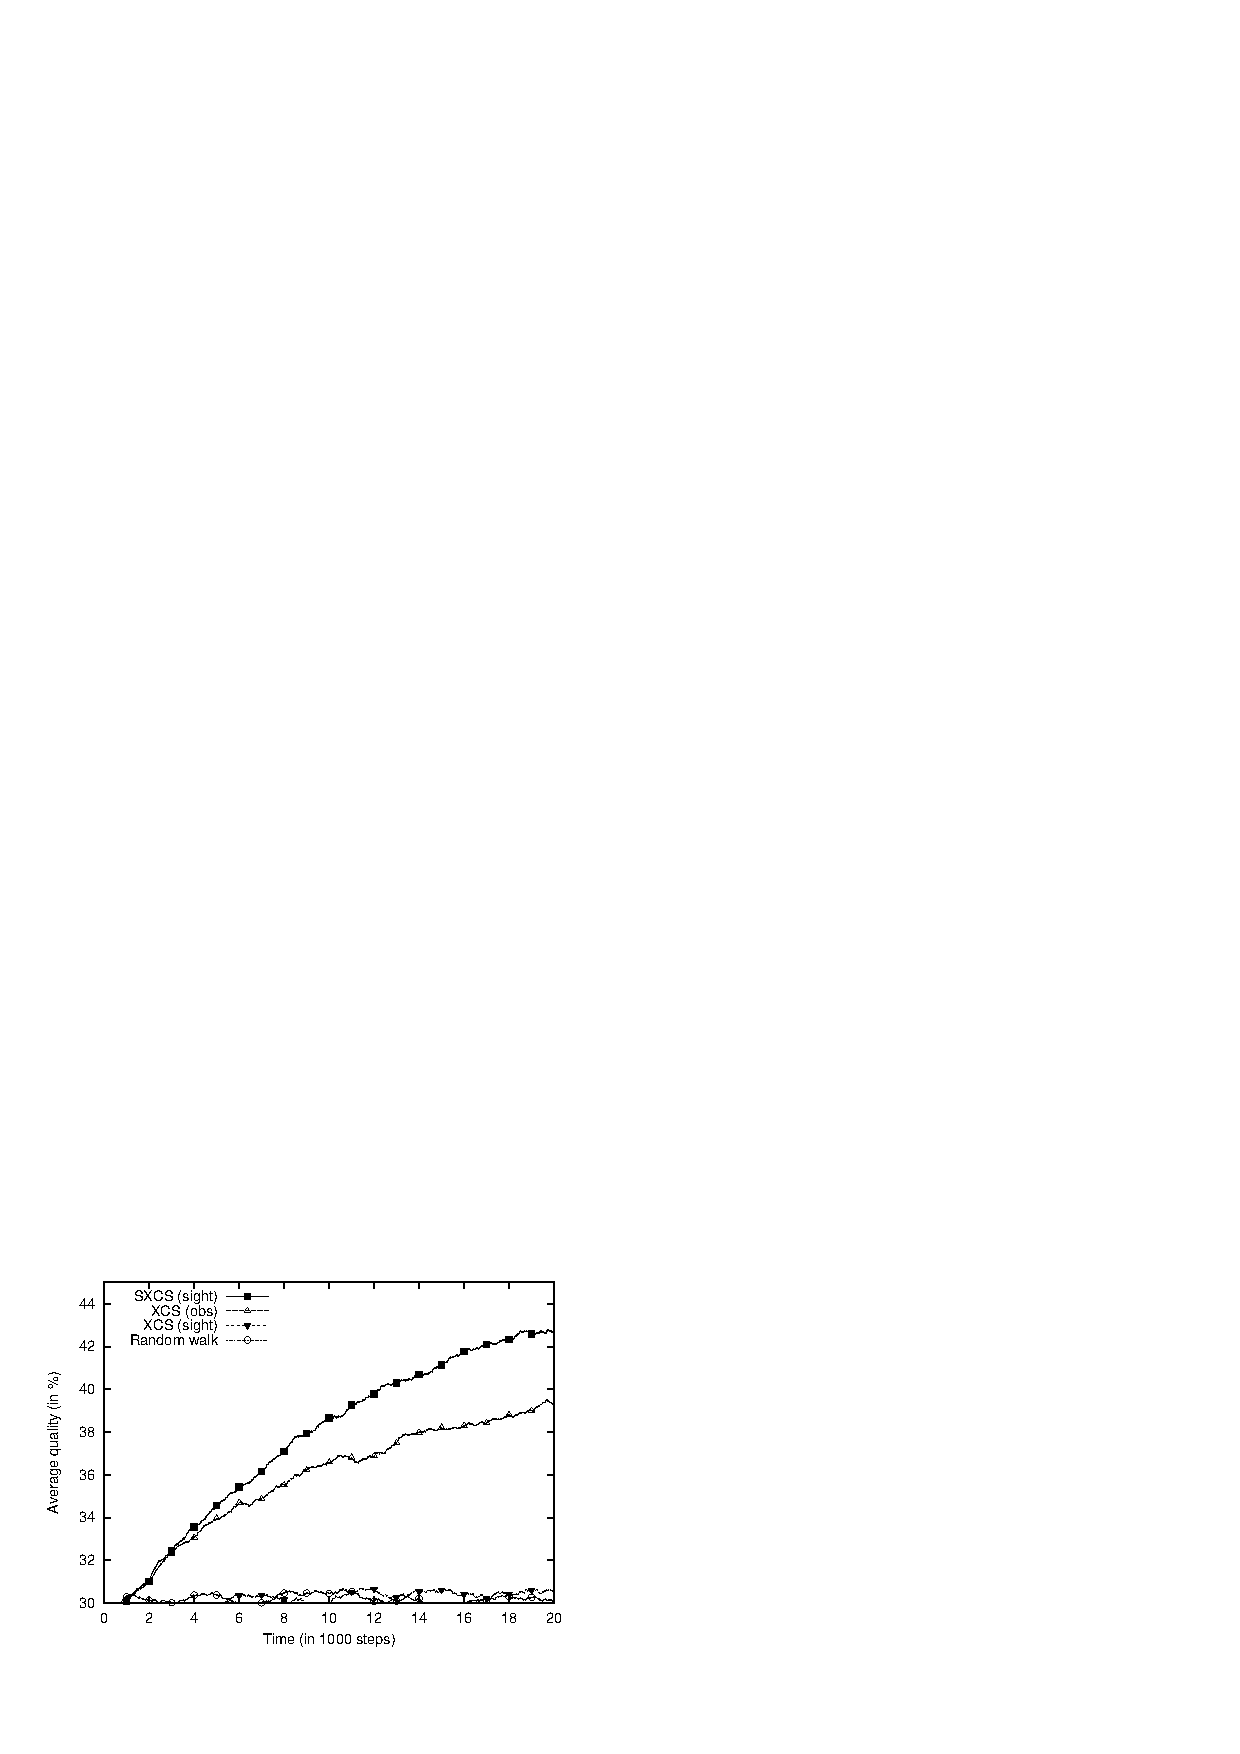
\includegraphics[width=0.24\textwidth]{plot_average_last_x_steps_goal_agent_observed-pillardir}}\hfill
  \subfigure[\emph{Pillar scenario} with a \emph{pre\-da\-tor-evading prey}]{
  	\label{figure:experiment-pillarint}
		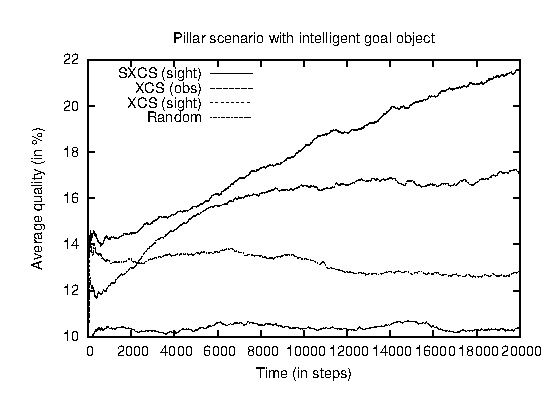
\includegraphics[width=0.24\textwidth]{plot_average_last_x_steps_goal_agent_observed-pillarint}}\hfill
  \subfigure[\emph{Random scenario} with an ob\-sta\-cle-evading prey]{
  	\label{figure:experiment-randdir}
		\includegraphics[width=0.24\textwidth]{plot_average_last_x_steps_goal_agent_observed-randdir}}\hfill
	\subfigure[\emph{Difficult scenario} with a \emph{blind\-ed prey}]{
		\label{figure:experiment-difficult}
		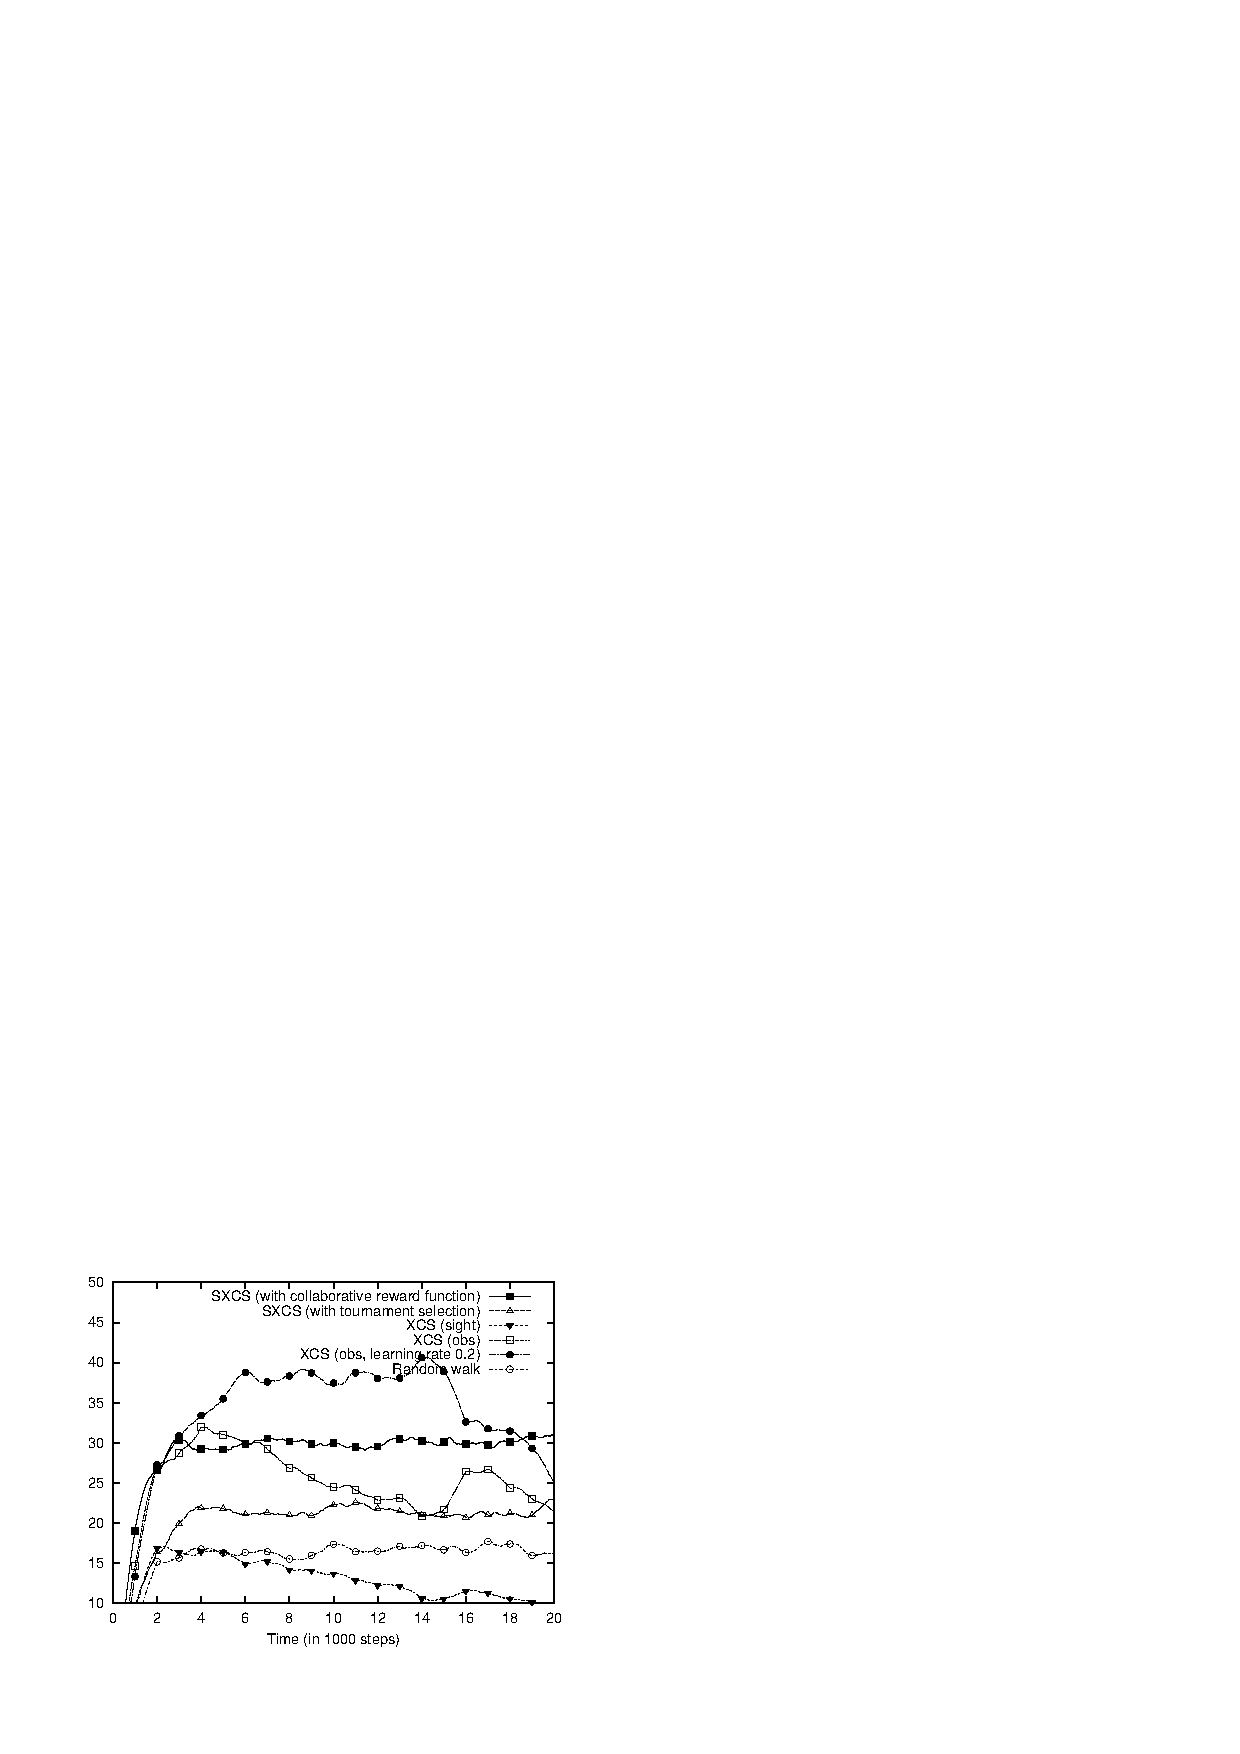
\includegraphics[width=0.24\textwidth]{plot_average_last_x_steps_goal_agent_observed-difficult}}
	\caption{\mathversion{bold}Comparison of the continuous average quality over time of different XCS variants}
	\label{figure:experiments}
\end{figure*}

\subsection{Discussion of Experimental Results}
\label{subsection:discussion-of-experimental-results}

As shown in Figures~\ref{figure:learning_rate} and \ref{figure:experiments}, \emph{XCS (sight)} is always inferior to \emph{XCS~(obs)}. Further tests on XCS plus different \emph{environmental reward functions} have led to the conclusion that XCS should not be combined with a reward function different to the global goal. Moreover, \emph{eventXCS} works well with strategies like \emph{selfish behavior (sight range)}, which is shown by the higher average quality of \emph{eventXCS} compared to \emph{XCS~(obs)} and an increased learning curve in the scenarios, depicted in Figures~\ref{figure:experiment-pillardir}, \ref{figure:experiment-pillarint}, and \ref{figure:experiment-randdir}. In the \emph{random scenario} with an obstacle-evading prey (see Figure~\ref{figure:experiment-randdir}), \emph{XCS} even shows no learning at all because of a relatively high percentage of wall collisions. Not depicted is the \emph{random scenario} with an predator-evading prey, the results are similar to the results of the \emph{pillar scenario} with the same type of prey.

% In addition, \emph{eventXCS} provides a significantly more stable learning, i.\,e., it shows no tendency of overlearning or unlearning, as shown in the \emph{random scenario} in Figure~\ref{figure:experiment-randdir}. Here, \emph{eventXCS} reaches significantly higher levels, while \emph{XCS (obs)} breaks down after 14,000 steps. To concluded, \emph{eventXCS} is clearly superior to \emph{XCS (obs)} in these three scenario configurations. 

Looking further on the \emph{difficult scenario}, it can be seen that \emph{eventXCS} clearly fails, no matter which \emph{learning rate} $\beta$ is used (see Figure~\ref{figure:learning_rate_difficult}). Since \emph{eventXCS} shares the same basic algorithm with \emph{XCS} and since the problem can be solved by choosing the classifiers more randomly using tournament selection (\emph{eventXCS~(ts)}), it points to a correctable flaw in the design of \emph{eventXCS}. Also including cooperative behavior (\emph{eventXCS~(coop,~ts)}) results in even better performance as the agents spread out more. While neither variant reaches the average quality level of \emph{XCS~(obs)}, they show a very stable learning, since \emph{XCS~(obs)} shows tendencies of over-learning or unlearning after 8\,000 steps or 14\,000 steps for $\beta = 0.2$ (see Figure~\ref{figure:experiment-difficult}). In general, it seems not surprising that \emph{XCS~(obs)} reaches better results than \emph{eventXCS}. \emph{XCS~(obs)} is designed to solve Maze scenarios, while \emph{eventXCS} has been modified to solve more open scenarios with a non-blinded prey, as investigated on the \emph{pillar} and the \emph{random scenario}. In summary, \emph{eventXCS} is clearly superior to \emph{XCS (obs)} in all four scenario configurations, it either reaches a better average quality or, with additional modifications, provides a similar quality with more stable learning.

% Alternative implementations of SXCS with \emph{tournament selection} on the other hand solve the problem but reach only a lower level as XCS with \emph{best selection} (see Figure~\ref{figure:experiment-difficult}). But as in the \emph{random scenario} with a predator-evading prey XCS seems to have problems with overlearning. Increasing the learning rate $\beta$ to $0.2$ increase the quality in short-term, but in long-term XCS still has problems while SXCS present a very stable learning curve. In connection with a collaborative base reward function SXCS is even able to outperform XCS in the long run.\\

% Figure~\ref{figure:experiment-heuristics} show a comparison between possible static strategies. Collaborative strategies have just a small advantage over simple greedy strategies.

% show the average percentage of time steps where the prey was in observation range (each averaged over the last 2000 steps). With an predator-evading prey SXCS clearly outperforms XCS, while in the case with the obstacle-evading prey both variants show a similar learning curve. In all cases increasing the base reward function for XCS from observation range to sight range resulted in worse results.\\
%The case with an obstacle-evading prey in the \emph{random scenario} is not displayed, none of the XCS variants are able to gain a significant advantage over a ``random walk'' strategy.

% In Section~\ref{section:experimental-results} it was shown that SXCS outperforms XCS in scenarios with few obstacles. This was mainly due to the fact that XCS is unable to handle base reward functions that differ from the global goal and because XCS seems to have problems reaching a stable level, possibly due to overlearning. 
%SXCS with \emph{best selection} showed serious problems in the \emph{difficult scenario} while it was able manage the problem with a more random \emph{tournament selection}. This points to a correctable flaw in the design of the algorithm (probably with the \emph{neutral events}). But other than XCS SXCS \emph{can} handle advanced base reward functions, e.g. with a collaborative element (evading other agents) which significantly helps for example in the \emph{difficult scenario} though this is probably due to the fact that it simply encourages agents to move away from other agents, explore the grid and move through the openings. But in the end SXCS was designed to follow and observe a moving prey, the \emph{difficult scenario} is more like a labyrinth where finding the prey in the first place is important.


\section{Experimental Results}
\label{section:experimental-results}

Many different design combinations of a reward function seem possible. This paper does not try to identify the best solution. Instead, it shows that there exists better implementations than the conventional XCS algorithm. Therefore, this paper concentrates on a comparison of XCS variants, as presented in Section~\ref{subsection:xcs-variants}. To properly compare these variants, it has been important to determine good parameter settings for each variant. While most of the standard values given in~\cite{BW02} and known as \emph{commonly used parameter settings} provide good results, some special settings need closer examination (see Section~\ref{subsection:xcs-parameters}). Thereby, thousands of different combinations have been tested and the parameter discussion could not completely be presented in here. Configurations that achieved a lower performance than a simple \emph{random walk} strategy are also omitted, since it is always difficult to argue, whether the increased performance of the predators' behavior is caused by an improved learning or by acting more equal to the \emph{random walk} strategy. Finally, selected results of a number of experiments are discussed in Section~\ref{subsection:discussion-of-experimental-results}.

\subsection{XCS Parameters}
\label{subsection:xcs-parameters}

The parameter \verb|maxStackSize| determines the stack overflow (and thus a \emph{neutral event}), as introduced in Section~\ref{subsection:events}. Similar to XCS' \emph{prediction discount} parameter $\gamma$, the optimal value is a compromise between several conflicting factors: Using larger values results in an inclusion of older -- maybe irrelevant -- actions in the reward of positive or negative events. Using smaller values can reduce the delay between an event and the actual reward, but it may also lead to a possible disregard of actions that are important for achieving the current event. In scenarios with fewer obstacles and more open space (\emph{random} and \emph{pillar scenario}), a value between $4$ and $8$ seems optimal (see Figures~\ref{figure:max-stack-size1} and \ref{figure:max-stack-size2}), while in more complex scenarios like the \emph{difficult scenario} significant larger values up to $32$ provide better results (see Figure~\ref{figure:max-stack-size3}). Additional experiments have shown that the size of the grid is also relevant, which points to a correlation between the optimal value and the average distance to the prey. As a compromise to achieve a better comparison, a value of \verb|maxStackSize| $ = 8$ has been used in all tests.

\begin{figure}[ht]
	\subfigure[\emph{Pillar scenario}]{ % with an \emph{ob\-sta\-cle-} and a \emph{pre\-da\-tor-evading prey}]{
		\label{figure:max-stack-size1}
		\includegraphics[width=0.15\textwidth]{plot_quality_maxstacksize1}}\hfill
	\subfigure[\emph{Random scenario}]{ % with an \emph{ob\-sta\-cle-} and a \emph{pre\-da\-tor-evading prey}]{
		\label{figure:max-stack-size2}
		\includegraphics[width=0.15\textwidth]{plot_quality_maxstacksize2}}\hfill
	\subfigure[\emph{Difficult scenario}]{ % with a \emph{blind\-ed prey}]{
		\label{figure:max-stack-size3}
		\includegraphics[width=0.15\textwidth]{plot_quality_maxstacksize3}}\hfill
	\caption{\mathversion{bold}Comparison of variants of \emph{eventXCS} with different \texttt{maxStackSize} values in different scenarios}
	\label{figure:max-stack-size}
\end{figure}

Another important parameter is the learning rate $\beta$. In a similar scenario in~\cite{1102281}, a value below the standard value is proposed (\(\beta = 0.02\)). The reason is that dynamic multi-agent systems can only be described by movement probabilities so that the learning process has to be slow and careful. Tests have shown that an optimal value ranges around $0.05$ in the \emph{pillar} and the \emph{random scenario} (see Figures~\ref{figure:learning_rate_pillar_dirchange}, \ref{figure:learning_rate_pillar_intelligent}, and \ref{figure:learning_rate_random_intelligent}) and between $0.6$ and $0.8$ in the \emph{difficult scenario} (see Figure \ref{figure:learning_rate_difficult}). To maintain comparability between the scenarios and to other XCS implementations, a $\beta$ value of \(0.05\) is used.
% in further tests. 
According to~\cite{BW02}, the maximum number of classifiers $N$ should be chosen large enough so that \emph{covering} only happens at the beginning.
% of a run. 
Here, tests have shown that a population size of $512$ classifiers fulfills this criterion. The classifier sets are filled with random classifiers~\cite{Butz2006}, but no significant difference could be seen compared to an empty initialization. Instead, sometimes a slower convergence has been observed, probably because the corresponding system has to unlearn irrelevant classifiers. The \emph{GA threshold} parameter $\theta_{\mathrm{GA}}$ is set to $25$, larger values reduces the quality of the algorithm. As \emph{eventXCS} itself makes use of a quadratic reward distribution, the parameter \emph{reward prediction discount} $\gamma$ is only needed to compare XCS to \emph{eventXCS}. However, tests have been inconclusive so that the standard value of $\gamma = 0.71$ is used. % Only \(\gamma = 1.0\) has shown significant differences in some cases. It seems that while a reduction of the transfer of the reward is needed, the actual value is of little importance. 
Only $\gamma = 1.0$ has shown significantly worse results in some cases, while the differences between the average qualities have been minimal for smaller values. % of $\gamma$. 
Other parameters, like the subsumption threshold $\theta_{\mathrm{sub}}$, the GA threshold $\theta_{\mathrm{GA}}$, and the mutation probability $\mu$, are initialized with default values ($20.0$, $25.0$, and $0.05$).

\begin{figure*}[ht]
  \subfigure[\emph{Pillar scenario} with an \emph{ob\-sta\-cle-evading prey}]{
		\label{figure:learning_rate_pillar_dirchange}
		\includegraphics[width=0.24\textwidth]{plot_quality_learning-pillardir}}\hfill
	\subfigure[\emph{Pillar scenario} with a \emph{pre\-da\-tor-evading prey}]{
		\label{figure:learning_rate_pillar_intelligent}
		\includegraphics[width=0.24\textwidth]{plot_quality_learning-pillarint}}\hfill
	\subfigure[\emph{Random scenario} with an \emph{ob\-sta\-cle-evading prey}]{
		\label{figure:learning_rate_random_intelligent}
		\includegraphics[width=0.24\textwidth]{plot_quality_learning-randdir}}\hfill
	\subfigure[\emph{Difficult scenario} with a \emph{blind\-ed prey}]{
		\label{figure:learning_rate_difficult}
		\includegraphics[width=0.24\textwidth]{plot_quality_learning-difficult}}
	\caption{\mathversion{bold}Comparison of different values for the learning rate $\beta$ for different XCS variants}
	\label{figure:learning_rate}
\end{figure*}

\begin{figure*}[ht]
  \subfigure[\emph{Pillar scenario} with an \emph{ob\-sta\-cle-evading prey}]{
  	\label{figure:experiment-pillardir}
  	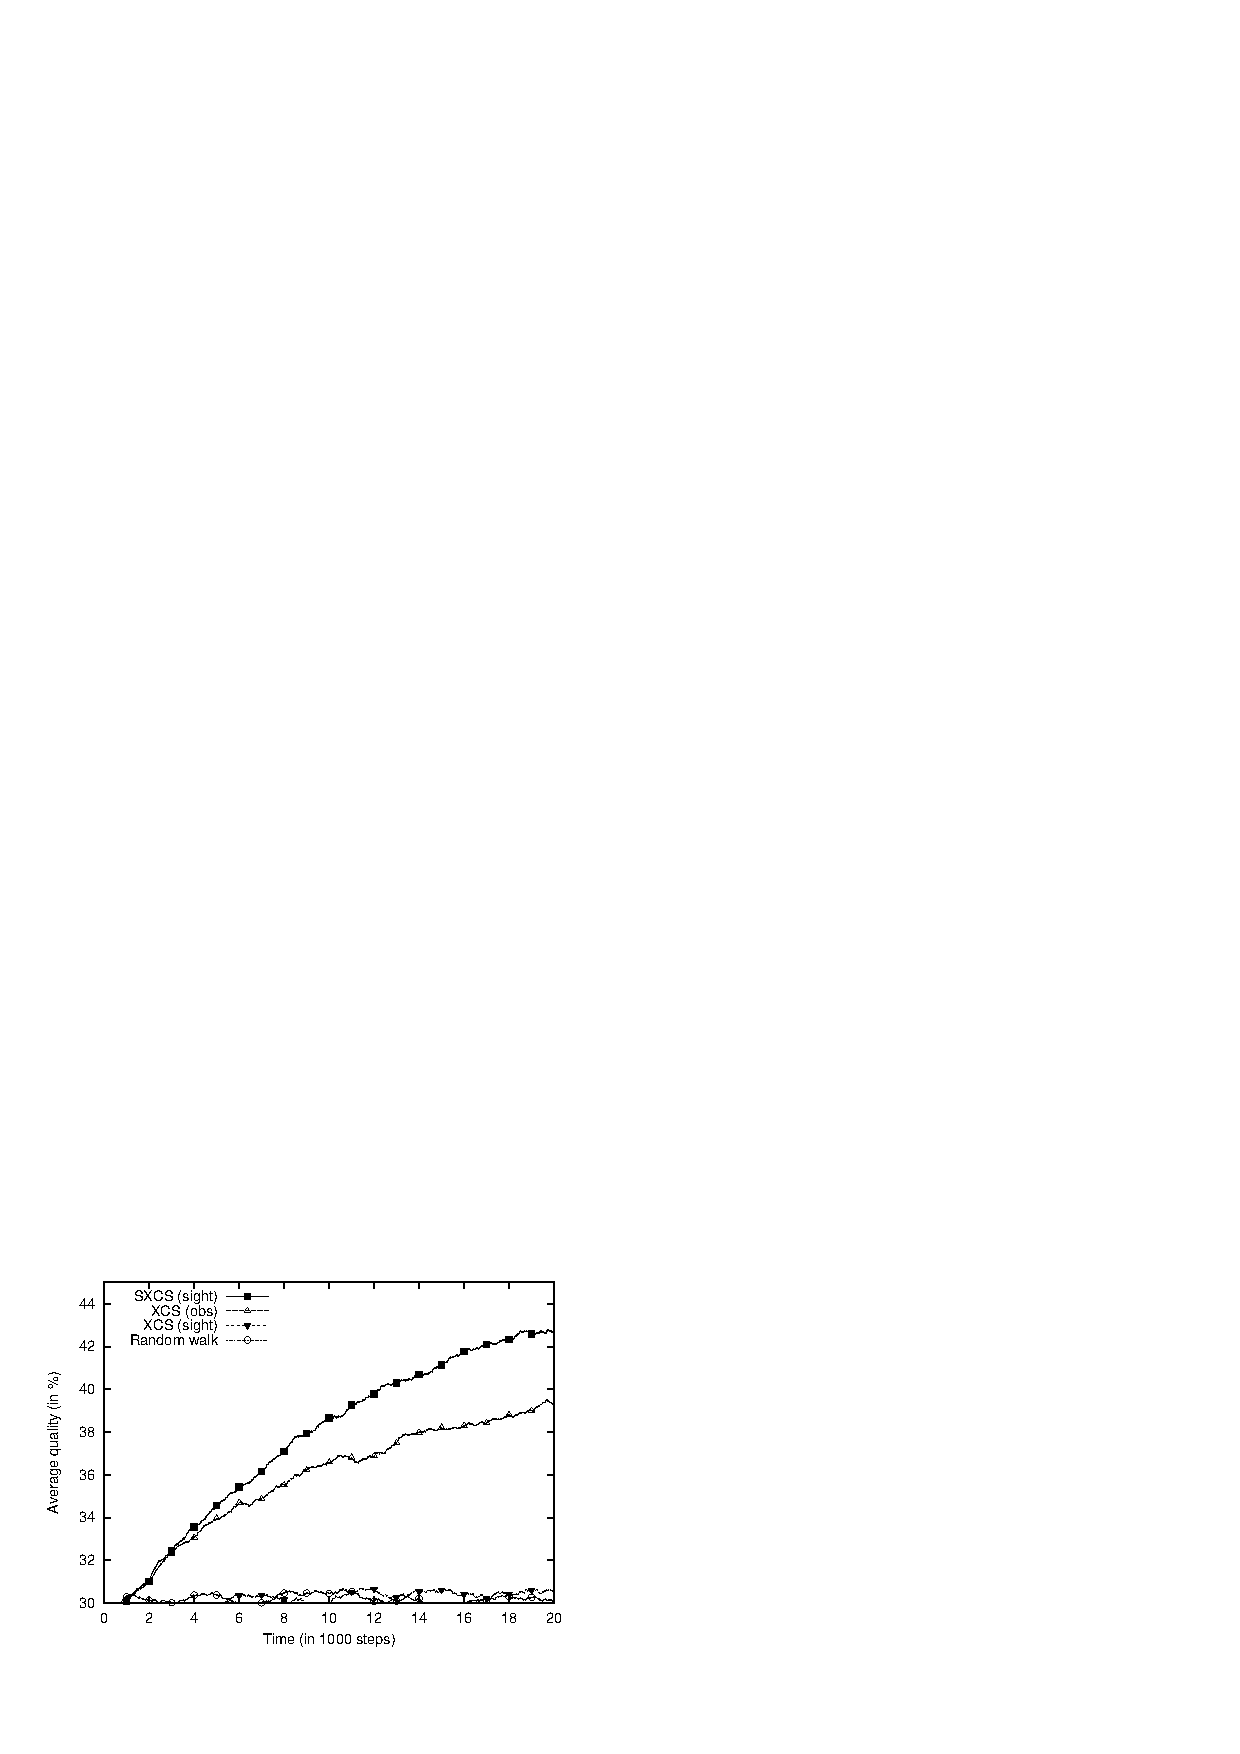
\includegraphics[width=0.24\textwidth]{plot_average_last_x_steps_goal_agent_observed-pillardir}}\hfill
  \subfigure[\emph{Pillar scenario} with a \emph{pre\-da\-tor-evading prey}]{
  	\label{figure:experiment-pillarint}
		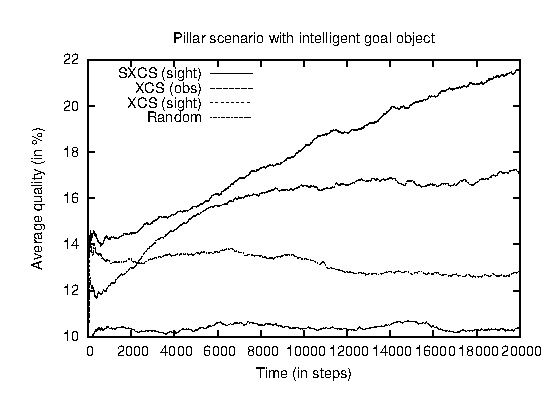
\includegraphics[width=0.24\textwidth]{plot_average_last_x_steps_goal_agent_observed-pillarint}}\hfill
  \subfigure[\emph{Random scenario} with an ob\-sta\-cle-evading prey]{
  	\label{figure:experiment-randdir}
		\includegraphics[width=0.24\textwidth]{plot_average_last_x_steps_goal_agent_observed-randdir}}\hfill
	\subfigure[\emph{Difficult scenario} with a \emph{blind\-ed prey}]{
		\label{figure:experiment-difficult}
		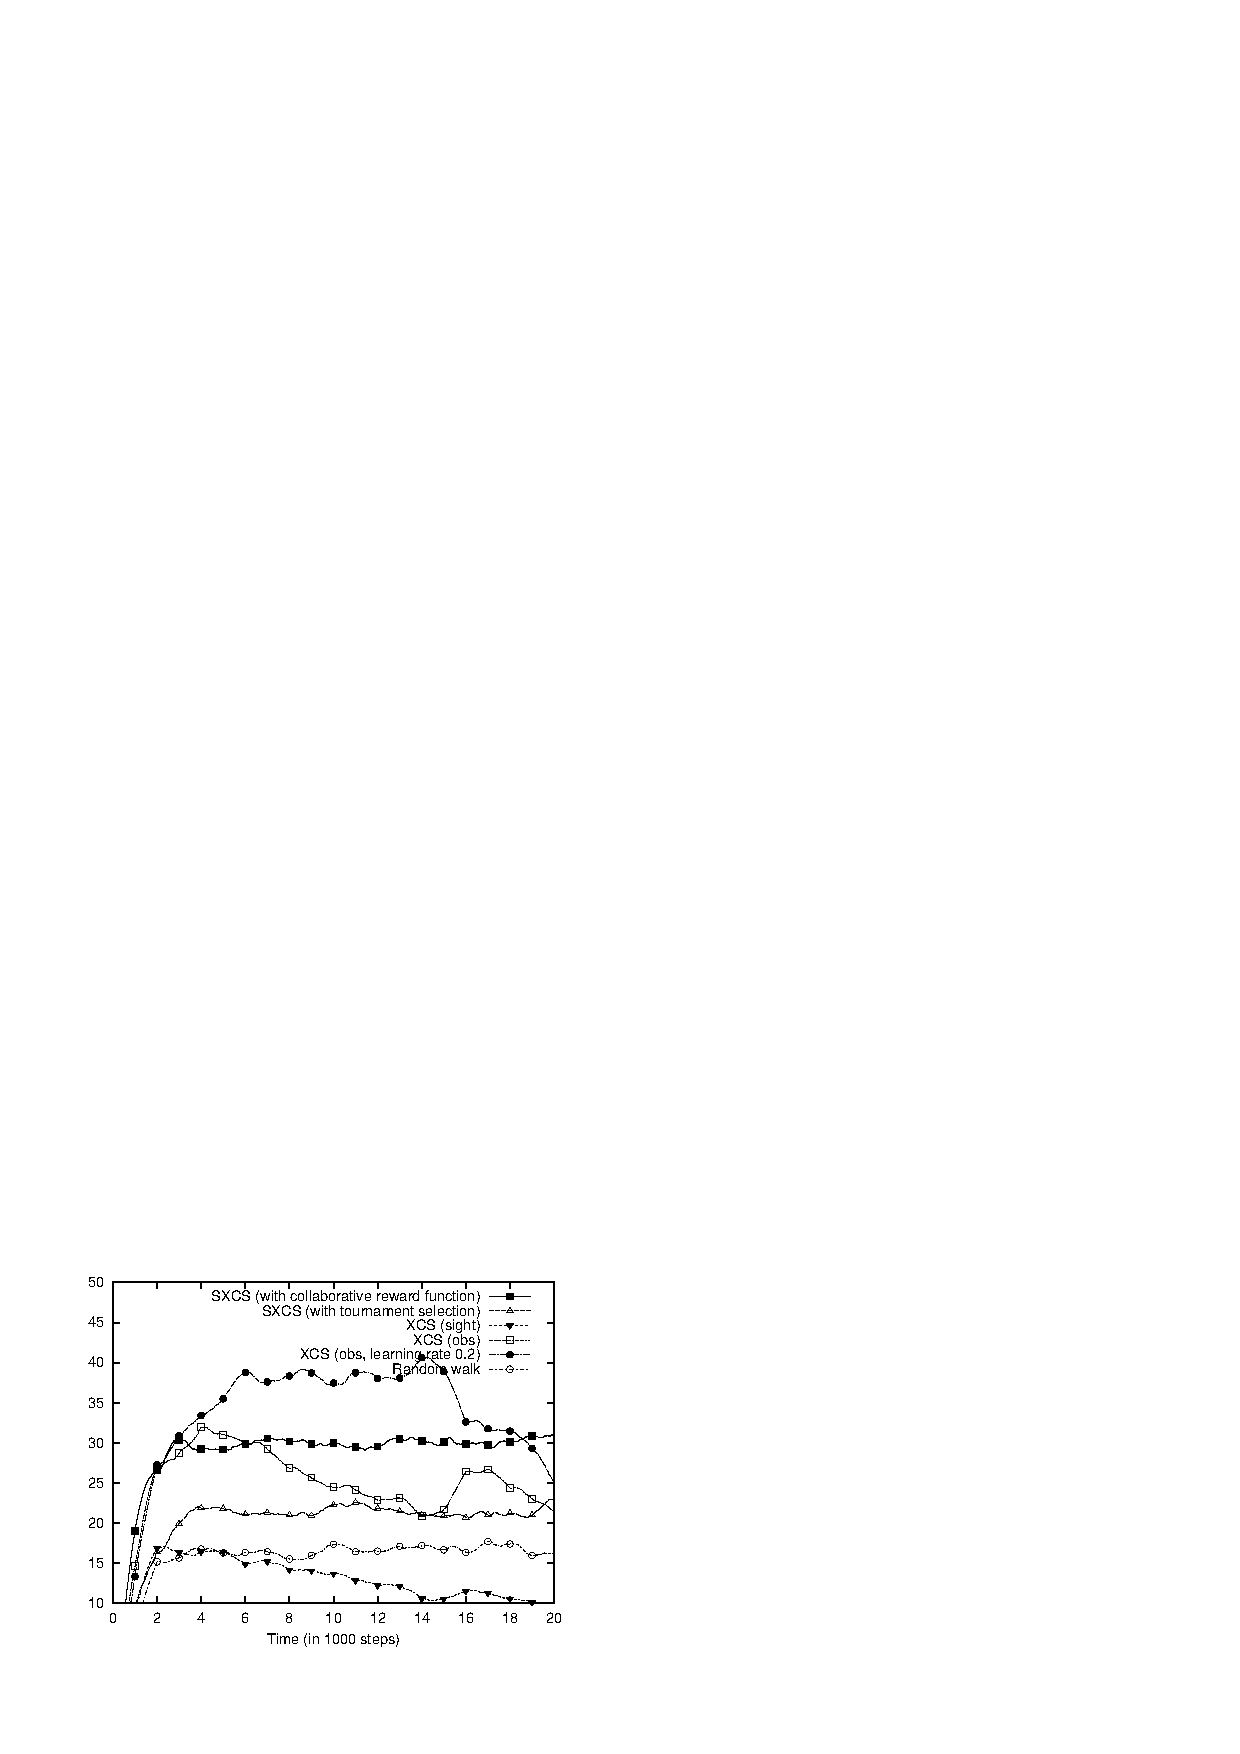
\includegraphics[width=0.24\textwidth]{plot_average_last_x_steps_goal_agent_observed-difficult}}
	\caption{\mathversion{bold}Comparison of the continuous average quality over time of different XCS variants}
	\label{figure:experiments}
\end{figure*}

\subsection{Discussion of Experimental Results}
\label{subsection:discussion-of-experimental-results}

As shown in Figures~\ref{figure:learning_rate} and \ref{figure:experiments}, \emph{XCS (sight)} is always inferior to \emph{XCS~(obs)}. Further tests on XCS plus different \emph{environmental reward functions} have led to the conclusion that XCS should not be combined with a reward function different from the global goal. Moreover, \emph{eventXCS} works well with strategies like \emph{selfish behavior (sight range)}, which is shown by the higher average quality of \emph{eventXCS} compared to \emph{XCS~(obs)} and an increased learning curve in the scenarios, depicted in Figures~\ref{figure:experiment-pillardir}, \ref{figure:experiment-pillarint}, and \ref{figure:experiment-randdir}. In the \emph{random scenario} with an obstacle-evading prey (see Figure~\ref{figure:experiment-randdir}), \emph{XCS} even shows no learning at all because of a relatively high percentage of wall collisions. Not depicted is the \emph{random scenario} with an predator-evading prey, the results are similar to the results of the \emph{pillar scenario} with the same type of prey.

Looking further on the \emph{difficult scenario}, it can be seen that \emph{eventXCS} clearly fails, no matter which \emph{learning rate} $\beta$ is used (see Figure~\ref{figure:learning_rate_difficult}). Since \emph{eventXCS} shares the same basic algorithm with \emph{XCS} and since the problem can be solved by choosing the classifiers more randomly using tournament selection (\emph{eventXCS~(ts)}), it points to a correctable flaw in the design of \emph{eventXCS}. Also including cooperative behavior (\emph{eventXCS~(coop,~ts)}) results in even better performance as the agents spread out more. While neither variant reaches the average quality level of \emph{XCS~(obs)}, they show a very stable learning, since \emph{XCS~(obs)} shows tendencies of over-learning or unlearning after 8\,000 steps or 14\,000 steps for $\beta = 0.2$ (see Figure~\ref{figure:experiment-difficult}). In general, it seems not surprising that \emph{XCS~(obs)} reaches better results than \emph{eventXCS}. \emph{XCS~(obs)} is designed to solve Maze scenarios, while \emph{eventXCS} has been modified to solve more open scenarios with a non-blinded prey, as investigated on the \emph{pillar} and the \emph{random scenario}. In summary, \emph{eventXCS} is clearly superior to \emph{XCS (obs)} in all four scenario configurations, it either reaches a better average quality or, with additional modifications, provides a similar quality with more stable learning.



%\section{Conclusion}
\label{section:conclusion}

% TODO bigger grid

A promising modified XCS approach has been investigated to overcome the drawbacks of the standard XCS algorithm concerning NOMDPs. The proposed idea is mainly based on expanding the local reward function and adding some kind of temporary memory, which stores past action sets and their corresponding reward values. Local payoffs can be delayed and analyzed later. Thus, the reward function reflects better the local agent's behavior. The experiments have shown that this new approach is superior to the standard XCS algorithm, mainly due to its ability to work well with advanced local reward functions, an ability, which XCS seemingly lacks. Besides improving the algorithm itself, future work will focus on an intelligent switching strategy between \emph{explore} (when no prey is in sight) and \emph{exploit phases} (when a predator is near by the prey). Further improvement is expected by an adaptive \emph{learning rate} $\beta$ and an adaptive \verb|maxStackSize| to fit the current scenario's needs. Finally, it seems interesting to test the \emph{eventXCS} approach on larger grids, on standard Maze scenarios, or other NOMDPs from literature.

% Cooperation (incorporated in the reward function) is more or less achieved through rejection and attraction. Predators reject each other, the prey attracts the predators. Thus, agents try to uniformly distribute on the grid and observation time of the prey seems to be maximized. In addition it is shown that the new XCS approach retains its ability to recognize local obstacle configurations in order to reach the goal object.
%In Section~\ref{section:experimental-results} it was shown that SXCS outperforms XCS in scenarios with few obstacles. This was mainly due to the fact that XCS is unable to handle base reward functions that differ from the global goal and because XCS seems to have problems reaching a stable level, possibly due to overlearning. 
%SXCS with \emph{best selection} showed serious problems in the \emph{difficult scenario} while it was able manage the problem with a more random \emph{tournament selection}. This points to a correctable flaw in the design of the algorithm (probably with the \emph{neutral events}). But other than XCS SXCS \emph{can} handle advanced base reward functions, e.g. with a collaborative element (evading other agents) which significantly helps for example in the \emph{difficult scenario} though this is probably due to the fact that it simply encourages agents to move away from other agents, explore the grid and move through the openings. But in the end SXCS was designed to follow and observe a moving prey, the \emph{difficult scenario} is more like a labyrinth where finding the prey in the first place is important.

% \begin{itemize}

% \item A good local evaluation function for the XCS can be constructed on the base of a heuristic with good performance (see Section~\ref{subsection:environment_reward_function}).

% TODO!
% \item By adding external memory that records the reward history (see Section~\ref{subsection:reward_distribution}) the newly created algorithm SXCS can solve the problem much better than XCS (see Section~\ref{section:experiments}).

% \item A variation of the learning rate $\beta$ can be successful depending on the scenario (see Section~\ref{subsection:learning_rate} and Section~\ref{subsection:xcs_difficult_scenario} for the difficult scenario respectively).

% \item Die Agenten mit XCS und SXCS haben deutliche Probleme mit Szenarien mit vielen Hindernissen (siehe Kapitel~\ref{subsection:tournament_factor_test}). TODO

% \item Ein dynamischer Wechsel der Auswahlart f�r Aktionen w�hrend eines Laufs kann sinnvoll sein, um die Zahl der blockierten Bewegungen zu verringern und das Zielobjekt besser verfolgen zu k�nnen (siehe Kapitel~\ref{subsection:analysis_random_scenario_xcs}). TODO

% \item XCS as well as SXCS can solve difficult scenarios with positions of interest significantly better than randomly moving agents. Under certain circumstances SXCS can solve this scenario even better than the heuristic on which its evaluation function is based on (see Section~\ref{subsection:xcs_difficult_scenario}).

% \end{itemize}

% binary function
% This causes some problems when trying to model the heuristic as it is impossible to distinguish situation with e.g. one other agent and four other agent in sight. Probably a better implementation would be to count the number of agents and return it as a reward. An additional problem surfaces in scenarios with a relatively low number of agents because the reward function returns 1 most of the time. This could harm the learning process.

% \begin{figure}[ht]
% \centerline{	
% \includegraphics[scale=0.75]{neutral_reward}
% }
% \caption{Schematic display of the reward distribution to the action sets after a neutral event (with \emph{base reward} = 1)}
% \label{figure:neutral_reward}
% \end{figure}

% In XCS wird lediglich die jeweils letzte \emph{action set} Liste aus dem vorherigen Schritt gespeichert. In der neuen Implementierung werden dagegen eine ganze Anzahl (bis zum Wert \emph{maxStackSize}) von \emph{action set} Listen gespeichert. Die Speicherung erlaubt zum einen eine Vorverarbeitung des \emph{reward} Werts anhand der vergangenen Schritte und auf Basis einer gr��eren Zahl von \emph{action set} Listen und zum anderen die zeitliche Relativierung einer \emph{action set} Liste zu einem Ereignis. Die \emph{classifier} werden dann jeweils r�ckwirkend anhand des jeweiligen \emph{reward} Werts aktualisiert, sobald bestimmte Bedingungen eingetreten sind.

% Bei der Benutzung eines solchen Stacks entsteht eine Zeitverz�gerung, d.h. die \emph{classifier} erhalten jeweils Informationen, die bis zu \emph{maxStackSize} Schritten zu alt sein k�nnen. Tritt beim Stack ein �berlauf auf, gab es also \emph{maxStackSize} Schritte lang keine �nderung des \emph{base reward} Werts mehr, dann wird abgebrochen und die \(\frac{maxStackSize}{2}\) �ltesten Eintr�ge werden vom Stack genommen. Alle diese Eintr�ge werden dabei vorher mit einem \emph{reward} Wert aktualisiert, der diesem \emph{base reward} Wert entspricht.

% In such a case 

% There are two drawbacks with this implementation: Firstly there is a time delay of the reward distribution because it is impossible to foresee when an event will occur. Secondly, in the case of a neutral event, the prediction of future events could be wrong and a new positive or negative event occurs shortly after the neutral event (see Figure~\ref{figure:neutral_reward}). Both points do not seem significant because the time delay, compared to the standard implementation with repetition of the problem, is very small and the erroneous reward distribution in the case of a neutral event could be corrected retroactively to a certain degree. On the other hand recording the history of rewards could provide a basis for a deeper analysis resulting in a better reward distribution than the one that is presented here.

% \subsection{Implementation of SXCS}

% The original implementation~\cite{But00} of XCS allows a modular setup of the environment so that the reward function (see Section~\ref{subsection:reward_function}) can be calculated in the environment module. As explained in Section~\ref{subsection:reward_distribution} and ~\ref{subsection:events} additional recording and analysis of the base reward generated by the reward function is necessary. Thus some parts of the code need to be rewritten resulting in the following modified version of the code:
% TODO Code?



\section{Conclusion}
\label{section:conclusion}

A promising modified XCS approach has been investigated to overcome the drawbacks of the standard XCS algorithm concerning NOMDPs. The proposed idea is mainly based on expanding the local reward function and adding some kind of temporary memory, which stores past action sets and their corresponding reward values. Local payoffs can be delayed and analyzed later. Thus, the reward function reflects better the local agent's behavior. The experiments have shown that this new approach is superior to the standard XCS algorithm, mainly due to its ability to work well with advanced local reward functions, an ability, which XCS seemingly lacks. Besides improving the algorithm itself, future work will focus on an intelligent switching strategy between \emph{explore} (when no prey is in sight) and \emph{exploit phases} (when a predator is near the prey). Further improvement is expected by an adaptive \emph{learning rate} $\beta$ and %an adaptive 
\verb|maxStackSize| to fit the current scenario's needs. Finally, it seems interesting to test the \emph{eventXCS} approach on larger grids, on standard Maze scenarios, or other NOMDPs from literature.

\bibliographystyle{abbrv}
%\bibliography{bib/sigproc}
\begin{thebibliography}{10}
\bibitem{BZ05}
A.~J. Bagnall and Z.~V. Zatuchna.
\newblock On the classification of {M}aze problems.
\newblock In {\em Foundations of Learning Classifier Systems}, volume 183 of
  {\em Studies in Fuzziness and Soft Computing}, pages 305--316. Springer,
  2005.

\bibitem{BJD86}
M.~Benda, V.~Jagannathan, and R.~Dodhiawala.
\newblock An optimal cooperation of knowledge sources: {A}n empirical
  investigation.
\newblock Technical Report BCS-{\-}G2010--{\-}28, Boeing Advanced Technology
  Center, Boeing Computing Services, 1986.

\bibitem{Butz2006}
M.~V. Butz.
\newblock {\em The {XCS} classifier system}, chapter~4, pages 51--64.
\newblock Springer, 2006.

\bibitem{BKLW04}
M.~V. Butz, T.~Kovacs, P.~L. Lanzi, and S.~W. Wilson.
\newblock Toward a theory of generalization and learning in {XCS}.
\newblock {\em IEEE Transactions on Evolutionary Computation}, 8(1):28--46,
  2004.

\bibitem{Butz2003}
M.~V. Butz, K.~Sastry, and D.~E. Goldberg.
\newblock Tournament selection: {S}table fitness pressure in {XCS}.
\newblock In {\em Proceedings of the Genetic and Evolutionary Computation
  Conference (GECCO 2003)}, volume 2724 of {\em LNCS}, pages 1857--1869.
  Springer, 2003.

\bibitem{BW02}
M.~V. Butz and S.~W. Wilson.
\newblock An algorithmic description of {XCS}.
\newblock {\em Soft Computing}, 6(3--4):144--153, 2002.

\bibitem{Hol75}
J.~H. Holland.
\newblock {\em Adaptation in natural and artificial systems}.
\newblock University of Michigan Press, 1975.

\bibitem{Hol76}
J.~H. Holland.
\newblock Adaptation.
\newblock In {\em Progress in Theoretical Biology IV}, pages 263--293. Academic
  Press, 1976.

\bibitem{HR78}
J.~H. Holland and J.~S. Reitman.
\newblock Cognitive systems based on adaptive algorithms.
\newblock In {\em Pattern-Directed Inference Systems}, pages 313--329. Academic
  Press, 1978.

\bibitem{1102281}
H.~Inoue, K.~Takadama, and K.~Shimohara.
\newblock Exploring {XCS} in multi-agent environments.
\newblock In {\em Proceedings of the 2005 Workshops on Genetic and Evolutionary
  Computation Conference (GECCO 2005)}, pages 109--111. ACM, 2005.

\bibitem{Miyazaki2}
S.~K. K.~Miyazaki.
\newblock On the rationality of profit sharing in multi-agent reinforcement
  learning.
\newblock In {\em Proceedings of the 4th International Conference on
  Computational Intelligence and Multimedia Applications (ICCIMA 2001)}, pages
  421--425. IEEE, 2001.

\bibitem{Kov02a}
T.~Kovacs.
\newblock Learning classifier systems resources.
\newblock {\em Soft Computing}, 6(3--4):240--243, 2002.

\bibitem{KL00}
T.~Kovacs and P.~L. Lanzi.
\newblock A bigger learning classifier systems bibliography.
\newblock In {\em Proceedings of the International Workshop on Learning
  Classifier Systems (IWLCS 2000)}, volume 1996 of {\em LNAI}, pages 213--249.
  Springer, 2000.

\bibitem{Lan98}
P.~L. Lanzi.
\newblock Adding memory to {XCS}.
\newblock In {\em Proceedings of the IEEE International Conference on
  Evolutionary Computation (CEC 1998)}, pages 609--614. IEEE, 1998.

\bibitem{Lan08}
P.~L. Lanzi.
\newblock Learning classifier systems: {T}hen and now.
\newblock {\em Evolutionary Intelligence}, 1(1):63--82, 2008.

\bibitem{LW00}
P.~L. Lanzi and S.~W. Wilson.
\newblock Toward optimal classifier system performance in non-{M}arkov
  environments.
\newblock {\em Evolutionary Computation}, 8(4):393--418, 2000.

\bibitem{RMB+06}
U.~Richter, M.~Mnif, J.~Branke, C.~M{\"{u}}ller-Schloer, and H.~Schmeck.
\newblock Towards a generic observer/controller architecture for organic
  computing.
\newblock In {\em INFORMATIK 2006 -- Informatik f{\"u}r Menschen!}, volume P-93
  of {\em LNI}, pages 112--119. Bonner K{\"o}llen Verlag, 2006.

\bibitem{SV00}
P.~Stone and M.~Veloso.
\newblock Multi-agent systems: {A} survey from a machine learning perspective.
\newblock {\em Autonomous Robots}, 8(3):345--383, 2000.

\bibitem{TTS01}
K.~Takadama, T.~Terano, and K.~Shimohara.
\newblock Learning classifier systems meet multi-agent environments.
\newblock In {\em Advances in Learning Classifier Systems}, volume 1996 of {\em
  LNAI}, pages 192--212. Springer, 2001.

\bibitem{Wil94}
S.~W. Wilson.
\newblock {ZCS}: {A} zeroth level classifier system.
\newblock {\em Evolutionary Computation}, 2(1):1--18, 1994.

\bibitem{Wil95}
S.~W. Wilson.
\newblock Classifier fitness based on accuracy.
\newblock {\em Evolutionary Computation}, 3(2):149--175, 1995.

\end{thebibliography}

\end{document}
